\chapter{Theory and Motivation}
\label{chap:theory}

\section{The Standard Model of Particle Physics}
\label{sec:theSM}

The \ac{SM} of fundamental interactions is a theory
which describes the electromagnetic, weak and strong nuclear interactions, often
represented as a collection of the elementary particles predicted by the theory.
The \ac{SM} has successfully described data from a wide range of experiments, and in the 
years prior to the LHC, all of the predicted elementary particles were verified 
except for one: the Higgs boson. This chapter briefly describes the theory
behind the \ac{SM} and the Higgs mechanism, before discussing previous
experimental results in \ac{SM} Higgs boson searches and outlining the theory
and motivation behind a possible extension to the \ac{SM} - the \ac{MSSM}.

\subsection{Particles and Forces} 
\label{sec:particlesandforces}

The \ac{SM} is a renormalisable quantum field theory, in which the constituents of
matter are represented as spin-$\frac{1}{2}$ fermions which interact with
forces mediated by spin-1 bosons. These interactions are described by a
Lagrangian which is invariant under $SU(3)_{C} \times SU(2)_{L} \times U(1)_{Y}$
symmetries. The $SU(3)_{C}$ part describes the strong interaction, mediated by
particles which carry colour charge (C). In these interactions, described by the
theory of \ac{QCD}~\cite{Griffiths:2008nx,Perkins:2000uq}, the force mediators are massless gluons
and the coloured fermions are the quarks. A notable property of QCD interactions
is confinement, in which the coupling strength decreases and the interaction
becomes asymptotically free at high energy, leading to quarks being bound at 
small distances in hadrons \cite{Gross:1973id,Politzer:1973fx}. The remaining fundamental fermions,
the leptons, do not carry colour charge and hence do not interact via the strong
force. Both the leptons and quarks participate in electroweak interactions,
which are governed by the $SU(2)_{L} \times U(1)_{Y}$ symmetry.

The electroweak symmetry describes the unified electromagnetic and weak
interactions~\cite{GlashowPartialSymmetries,WeinbergModelOfLeptons,SalamNobelSymposium}, 
and was one of the major achievements of the twentieth
century in the \ac{SM}. In electroweak theory the quantum numbers are
weak isospin $t_{1,2,3}$ and hypercharge $y$. These are related to the
electric charge Q as: 

\begin{equation}
Q = t_{3} + \frac{y}{2}
\end{equation}

The gauge fields associated with these quantum numbers are the three weak isospin fields,
$W_{\mu}^{i}$, $i = 1,2,3$, and the hypercharge field $B_{\mu}$. The weak
isospin fields act on doublets: 

\begin{equation}
\psi_{L} =  \begin{pmatrix} u_{i} \\ d_{i} \end{pmatrix}_{L} ,   
\begin{pmatrix} \nu_{i} \\ {l_{i}} \end{pmatrix}_{L}
\end{equation}

where $u_{i}$ are the up-type quarks ($u,c,t$), $d_{i}$ are the down-type quarks
($d,s,b$), $l_{i}$ are the charged leptons ($e,\mu,\tau$) and $\nu_{i}$ are the
corresponding neutrinos ($\nu_{e},\nu_{\mu},\nu_{\tau}$). The index $i$ indicates first, second or third
generation fermions. The subscript $L$ indicates that the doublets correspond to
the left handed projection of the fermions. The weak force only interacts with
left handed fermions, and as such is maximally parity violating. The right
handed projections $\psi_{R}$
transform as singlet states, which are invariant under $SU(2)_{L}$.

The physical $\gamma, \PZ$ and $\PWpm$ bosons result from mixing between the gauge
fields:

\begin{equation}
\begin{pmatrix} A_{\mu} \\ Z_{\mu}^{0} \end{pmatrix} = 
\begin{pmatrix} \cos{\theta_{W}} & \sin{\theta_{W}} \\ -\sin{\theta_{W}} &
\cos{\theta_{W}} \end{pmatrix} . 
\begin{pmatrix} B_{\mu} \\ W_{\mu}^{3} \end{pmatrix}
\end{equation}

where $A_{\mu}$ is the photon field, $Z_{\mu}^{0}$ is the $\PZ$ field
and $\theta_{W}$ is the weak mixing angle,
which can be related to the couplings of the weak neutral ($g$) and electromagnetic
interactions ($g'$) as $\theta_{W}=\tan^{-1}{\frac{g'}{g}}$. The fields
corresponding to the $\PWpm$ bosons are related to the weak isospin fields as
$W_{\mu}^{\pm} = (1/\sqrt{2})(W_{\mu}^{1} \mp W_{\mu}^{2})$. Weak neutral
currents were discovered at the Gargamelle bubble chamber experiment in CERN in
1973 \cite{Hasert:1973ff}, and the $\PZ$ and $\PWpm$ bosons themselves were
discovered by the UA1 and UA2 collaborations at CERN in
1983~\cite{Arnison:1983rp,Banner:1983jy,Arnison:1983mk,Bagnaia:1983zx}.

Crucially, this leads to a Lagrangian which doesn't contain any mass terms.
Gauge mass terms of the form $-M^{2}W_{\mu}W^{\mu}$ break the gauge invariance
of the Lagrangian. Similarly fermion mass terms of the form
$-m\overline{\psi}\psi = -m(\overline{\psi_{R}}\psi_{L} +
\overline{\psi_{L}}\psi_{R})$, where $\overline\psi$ indicates the adjoint of
the field $\psi$, contain field pairs of left and right handed components which transform differently
under the $SU(2)_{L}$ and $U(1)_{Y}$ groups, and so also break gauge invariance.
Experimental results confirm the photon to be massless, but the $\PW$ and $\PZ$
bosons have finite masses of $\approx80.4~\GeV$ and $\approx91.2~\GeV$
respectively, and the fermions also have a range of finite masses~\cite{PDG}. As
such the electroweak symmetry must be spontaneously broken. The mechanism of
electroweak symmetry breaking in the \ac{SM} is the Higgs mechanism.

\subsection{The Higgs Mechanism in the Standard Model}
\label{sec:SMHiggs}

A symmetry in a quantum field theory is spontaneously broken when the Lagrangian
itself remains invariant whilst the vacuum state does
not~\cite{AitchisonGaugeTheories}. For electroweak
theory, this is achieved by introducing a complex scalar field which attains a
non-zero vacuum expectation value (VEV)
\cite{Higgs:1964ia,Higgs:1964pj,Guralnik:1964eu,Higgs:1966ev,Kibble:1967sv}. 
This field is an $SU(2)$ doublet, defined as:
\begin{equation}
\phi = \begin{pmatrix}\phi^{+} \\ \phi^{0} \end{pmatrix}
\end{equation}
The electroweak Lagrangian can be written in the following simple form:
\begin{equation}
\mathcal{L}_{EW} = -\frac{1}{4}(\mathbf{F_{\mu\nu}}\cdot\mathbf{F^{\mu\nu}} +
G_{\mu\nu}G^{\mu\nu}), 
\end{equation}
where $\mathbf{F_{\mu\nu}}$ and $G_{\mu\nu}$ are the weak isospin and field strength
tensors respectively, related to the fields as:
\begin{equation}
\mathbf{F_{\mu\nu}} = \partial_{\mu} \mathbf{W_{\nu}} - \partial_{\nu}\mathbf{W_{\mu}} -
g\mathbf{W_{\mu}} \times \mathbf{W_{\nu}} , 
\end{equation}
where $\mathbf{W_{\mu}}= (W_{\mu}^{1},W_{\mu}^{2},W_{\mu}^{3})$. Introducing the
complex scalar field $\phi$ yields an additional term of the form:
\begin{equation}
\mathcal{L_{\phi}} = (D_{\mu}\phi)^{\dagger}(D^{\mu}\phi) - V(\phi), \\ 
\text{with} \quad D_{\mu} = \partial_{\mu} - \frac{1}{2}(igT_{i}W_{\mu}^{i} - ig'B_{\mu}),
\end{equation}
where $T_{i}$ are the $SU(2)$ group generators. The term $V(\phi)$ is the
potential term, given by:
\begin{equation}
V(\phi) = \lambda(\phi^{\dagger}\phi)^{2} - \mu_{SM}\phi^{\dagger}\phi,
\end{equation}
where $\lambda$ and $\mu_{SM}$ are constants parametrising the self-interactions
and masses of the scalar fields. The vacuum states correspond to the minima of
$V(\phi)$ with expectation values of $\bra{0}\phi\ket{0}$, which are given by:
\begin{equation}
\bra{0}\phi\ket{0} = \frac{1}{\sqrt{2}} \begin{pmatrix}0 \\ v \end{pmatrix}, \\
\text{with} \quad v=\sqrt{\frac{\mu_{SM}^{2}}{\lambda}}.
\end{equation}
To obtain the physical particles, perturbations around the vacuum state are
considered. If $\theta_{i}$ and $H_{SM}$ represent small variations in the four
degrees of freedom of the field $\phi$ then:
\begin{equation}
\phi = \exp(-i\theta_{i}T^{i}/2v)\frac{1}{\sqrt{2}}\left(\frac{0}{v+H_{SM}} \right)
\end{equation}
An appropriate gauge transformation can set the phase fields $\theta_{i}$ to be
zero, leaving only $H_{SM}$. Inserting this into the Lagrangian, $H_{SM}$ is
identified as a scalar field with mass $\sqrt{2}\mu_{SM}$ and the $W_{\mu}^{\pm}$
and $Z_{\mu}^{0}$ fields acquire mass terms $m_{\PW}$ and $m_{\PZ}$ related by:
\begin{equation}
m_{\PW} = m_{\PZ}\cos{\theta_{W}}=\frac{gv}{2}.
\label{eq:vaccummw}
\end{equation}
Fermion mass terms are introduced via Yukawa interactions between the fermion
and Higgs fields, with the form:
\begin{equation}
-\lambda_{f}( \overline{\psi_{L}}\phi\psi_{R} +
\overline{\psi_{R}}\phi\psi_{L}),  
\label{eq:HiggsCoupling}
\end{equation}
where $\lambda_{f}$ is the coupling for each fermion. The values $\lambda_{f}$ 
are proportional to the mass of the fermion $m_{f}$, such that heavier fermions have stronger
coupling to the Higgs boson. The \ac{SM} does not predict values for these
couplings, but they can be determined using the experimentally measured masses
of the fermions. The experimentally measured $\PW$ and $\PZ$ masses can be used
alongside the measured value of the fine structure constant to determine
$\sin{\theta_{W}}$, $v$ and $g$, but the value of $\mu_{SM}$ cannot be
predicted. Hence the mass of the Higgs boson associated with the Higgs field,
$m_{\PH}=\sqrt{2}\mu_{SM}$, is not predicted by the \ac{SM}.

\subsection{Searching for the SM Higgs boson}
\label{sec:LHCSMHiggs}

Since the mass of the Higgs boson is not directly predicted by the \ac{SM},
searches covering a wide range of potential masses must be performed.
The Higgs boson is produced in particle accelerators and searched for via a signature 
resulting from its decay to either fermions or bosons. The coupling of the
Higgs to a particular final state is determined as in equation~\ref{eq:HiggsCoupling} and
depends on both the mass of the Higgs boson and the mass of the final state
particles. 

Production of the Higgs boson occurs via the processes shown in
figure~\ref{fig:SMFeynmanDiagrams}: gluon-gluon fusion, \ac{VBF} and associated
production with either a vector boson or a pair of top quarks. The Higgs does
not couple directly to gluons since they are massless, and hence the gluon
fusion process proceeds via a quark loop. All four of these dominant production modes are
accessible at the LHC. 

\begin{figure}[htbp]
\subfloat[]{
   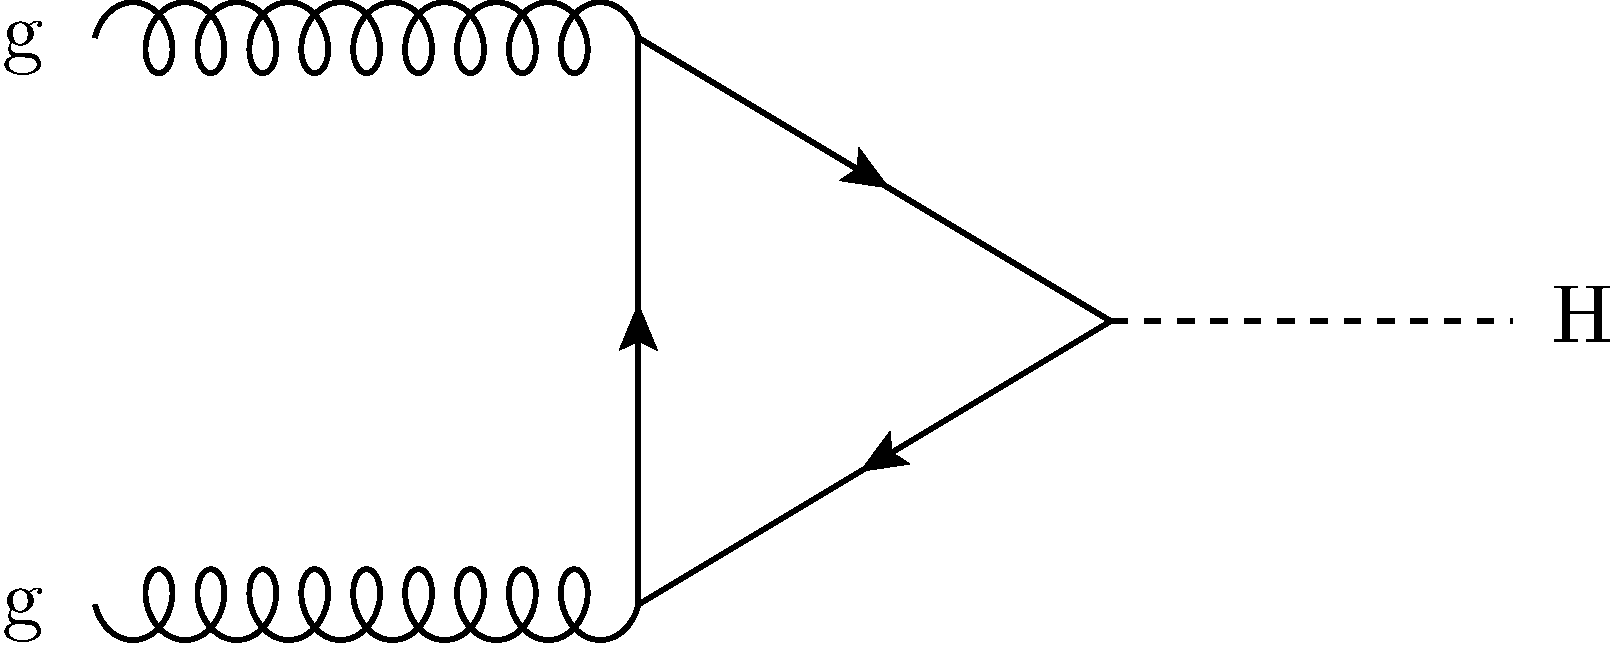
\includegraphics[width=0.48\textwidth]{plots/theory/feynman_ggH.pdf}}
\subfloat[]{
   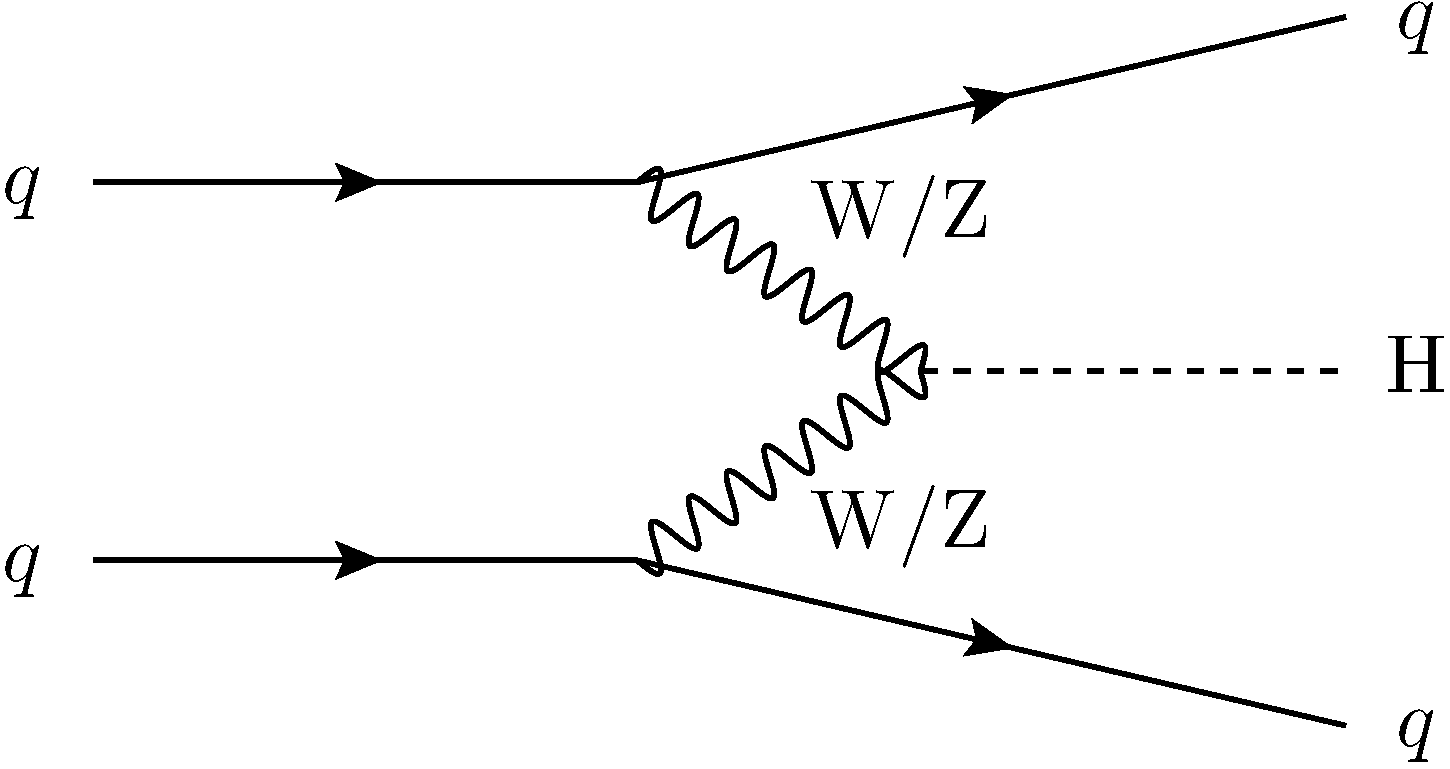
\includegraphics[width=0.4\textwidth]{plots/theory/feynman_qqH.pdf}}

\subfloat[]{
   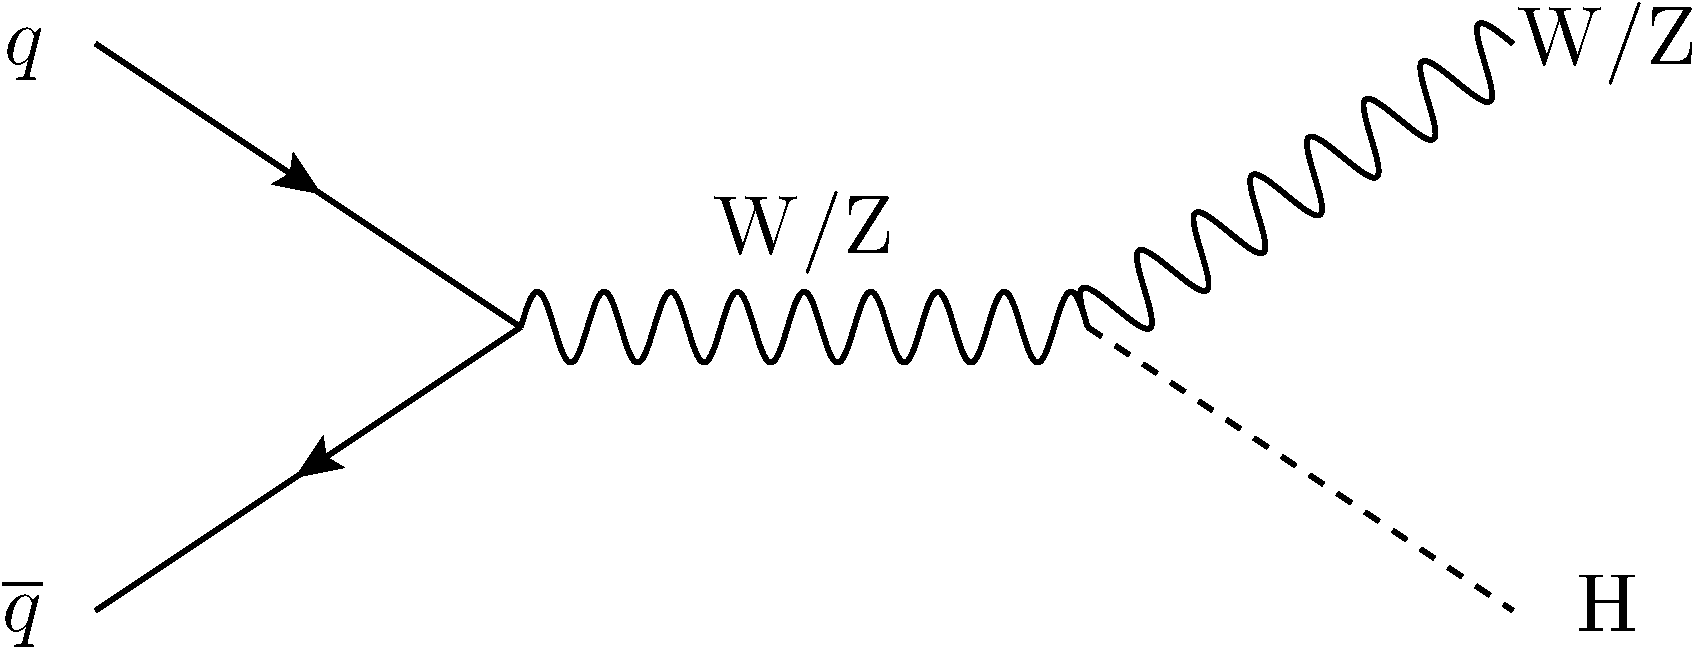
\includegraphics[width=0.48\textwidth]{plots/theory/feynman_VH.pdf}}
\subfloat[]{
   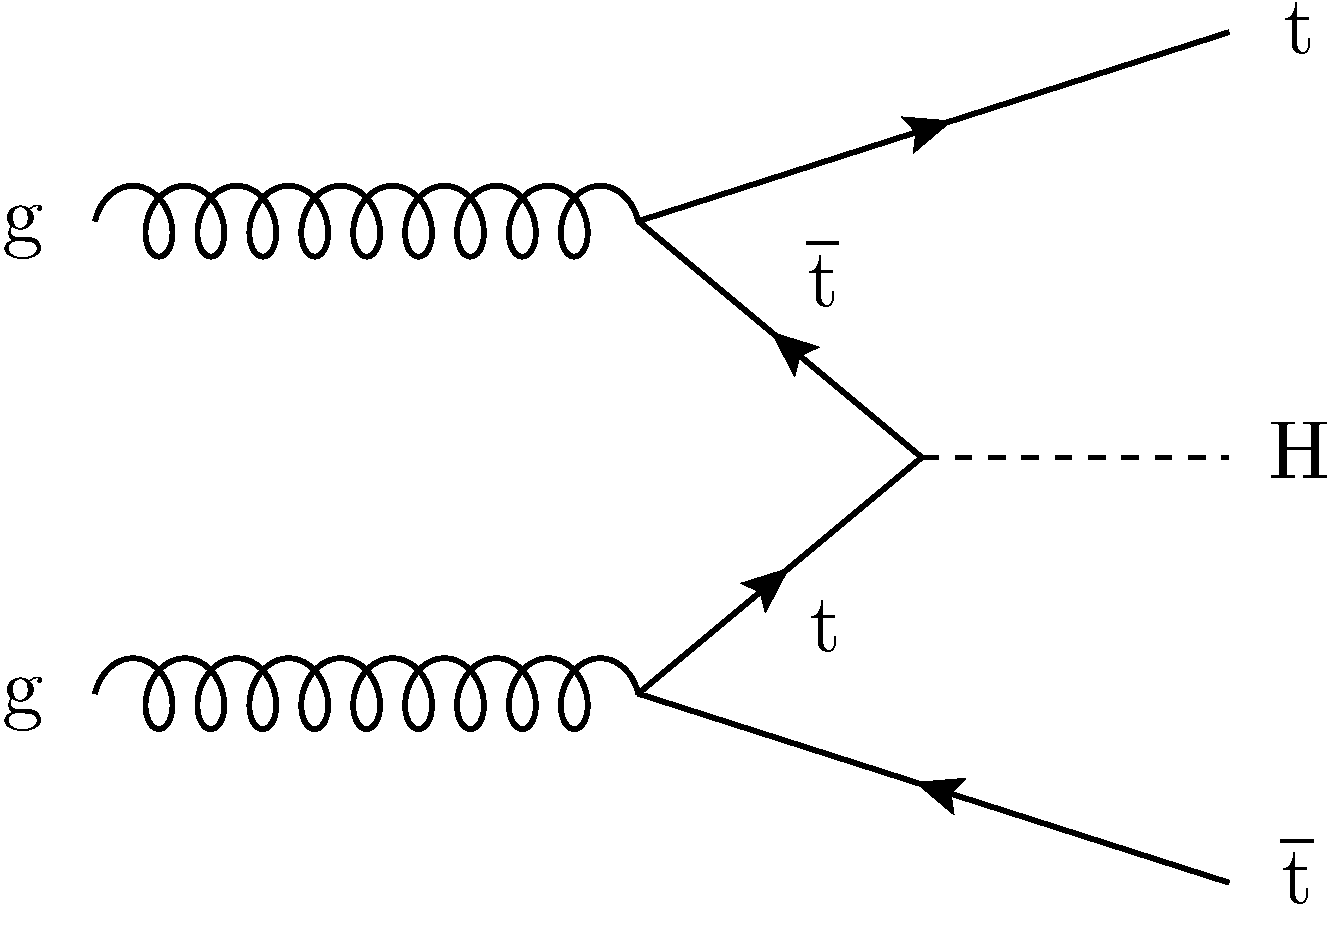
\includegraphics[width=0.4\textwidth]{plots/theory/feynman_ttH.pdf}}
\caption[Feynman diagrams for the dominant production processes of the SM Higgs
boson.]{Feynman diagrams for the dominant production processes of the SM Higgs
boson. Top left is gluon fusion, top right vector boson fusion, bottom shows
associated production with (left) vector bosons and (right) top quarks.}
\label{fig:SMFeynmanDiagrams}
\end{figure}

Previous searches for the Higgs boson were carried out at LEP and the
Tevatron. The LEP experiment collided electrons and positrons at centre of mass
energies ($\sqrt{s}$) between $90$ and $209\,\GeV$. In such collisions the Higgs
boson is predominantly produced in association with a $\PZ$ boson, a process
referred to as ``Higgsstrahlung''. The decay channels used were predominantly decays
to $\Pqb\Paqb$ and $\Pgtp\Pgtm$ pairs. The fact that the Higgs boson was not
observed at LEP yields the exclusion of masses with $m_{\PH}<114.4\,\GeV$ at the
95\% \ac{CL} \cite{Barate:2003sz}. Searches were also performed by the CDF and D0 Collaborations at
the Tevatron accelerator, which collided protons and antiprotons with
$\sqrt{s}=1.96\,\TeV$. The searches were performed in a mass range of
$90$--$200\,\GeV$ and focussed on decays into $\Pqb\Paqb$, $\PWp\PWm$,
$\gamma\gamma$ and $\Pgtp\Pgtm$ pairs, with  $\Pqb\Paqb$ and $\PWp\PWm$ offering
the highest sensitivity. The combined results from the Tevatron yielded
exclusions of $m_{\PH}$ in the ranges $90$--$109\,\GeV$ and $140$--$184\,\GeV$
\cite{Aaltonen:2013kxa}. The results of such direct searches
can be combined with precision measurements of electroweak observables at LEP
and by the SLAC Large Detector (SLD) to constrain the mass of the Higgs
boson to $94^{+29}_{-24}\,\GeV$ \cite{lepewwg}, 
where the uncertainty incorporates experimental effects only.

The LHC provides a higher centre of mass energy than the Tevatron, and so
gives access to higher cross-sections and a wider range of Higgs masses. Figure
\ref{fig:SMHiggsXS} indictates the cross-sections of the different production
processes, for proton-proton collisions at $\sqrt{s}=8~\TeV$ as used during the 
2012 operating period of the LHC. The gluon fusion production process dominates 
over the others by at least one order of magnitude in cross-section. 
Despite this, the other production modes are useful since have specific 
topologies which can be exploited in the selection of signal-like events. 
The \ac{VBF} process is characterised by the two outgoing quarks which
hadronise to form jets with high momentum, typically found in the forward
detector region. Production via the associated production process consists of a vector
boson or a pair of top quarks in the final state, yielding multi-lepton and 
multi-jet final states with reduced backgrounds from other \ac{SM} processes.

\begin{figure}[htbp]
   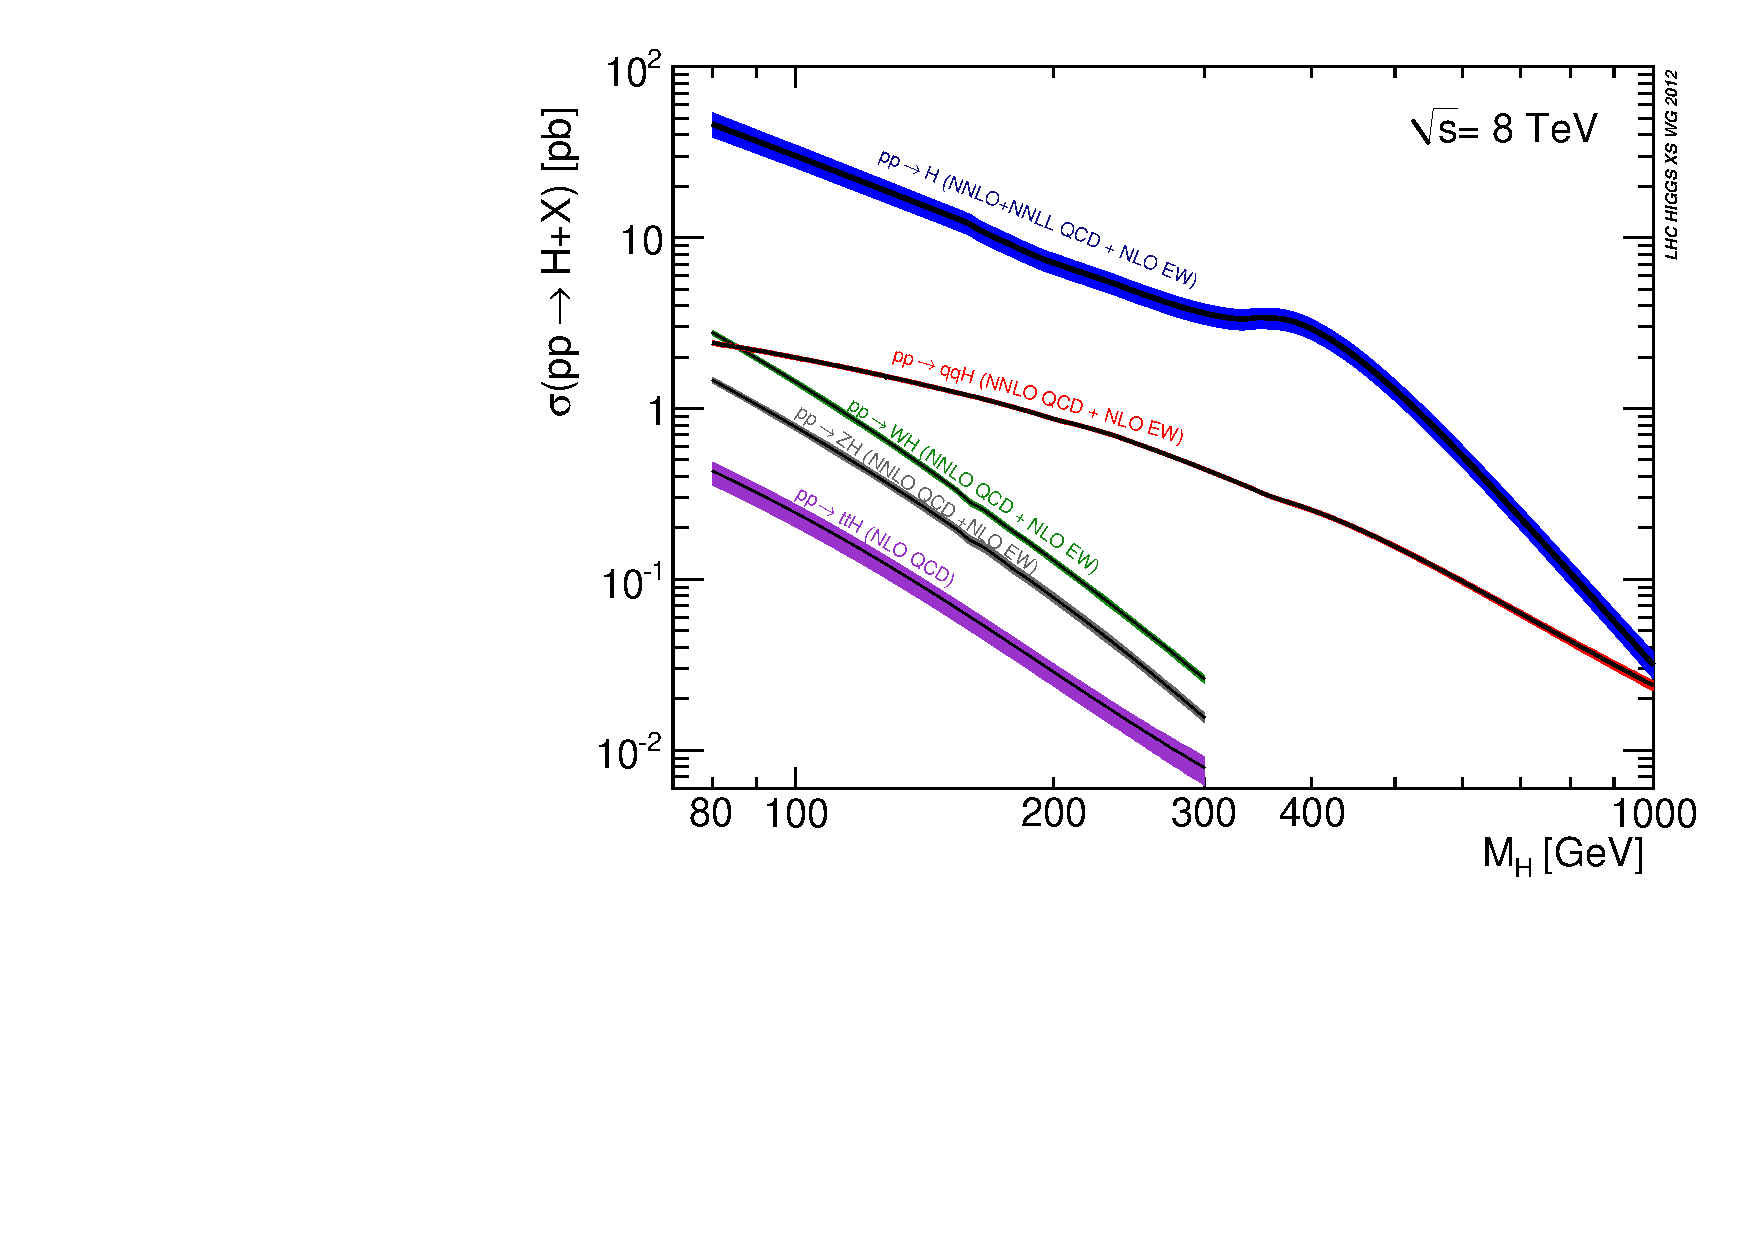
\includegraphics[width=0.7\textwidth]{plots/theory/Higgs_XS_8TeV_lx.pdf}
\caption[Cross sections for Higgs production processes at $\sqrt{s}=8~\TeV$ for
a range of Higgs boson masses.]{Cross sections for Higgs production processes at $\sqrt{s}=8~\TeV$ for
a range of Higgs boson masses $m_{\PH}$ \cite{Heinemeyer:2013tqa}. Across the
mass range the gluon-fusion mode dominates, followed by the vector boson fusion
and associated production modes.}
\label{fig:SMHiggsXS}
\end{figure}

The branching fractions to the different decay channels are shown in
figure \ref{fig:SMHiggsBRs} for a range of possible Higgs masses. At low Higgs
boson masses, a variety of different decay channels are accessible. The decay
into two photons occurs via a fermion loop, and decays to $\PWp\PWm$, $\PZ\PZ$,
$\Pqb\Paqb$ and $\Pgtp\Pgtm$ pairs are also possible. At higher Higgs masses
above $130~\GeV$, the decays into $\PWp\PWm$, $\PZ\PZ$ are more kinematically
favourable and hence dominate. In the discovery of a Higgs boson, identication of
any of these decay channels is important, but the most sensitive channels for
discovery in the low mass region are $\Pphoton\Pphoton$ and $\PZ\PZ$ due to
their clean signatures. However, upon discovery of a Higgs boson, decays into 
fermions are particularly important
to establish the Yukawa couplings. In fermionic decays, the decay into
$\Pqb\Paqb$ dominates with a branching fraction of $\sim 80\%$ in this mass
range. However, this final state is difficult to disentangle from the large QCD
jet background at the LHC, meaning that the $\Pgtp\Pgtm$ has higher sensitivity.

\begin{figure}[htbp]
   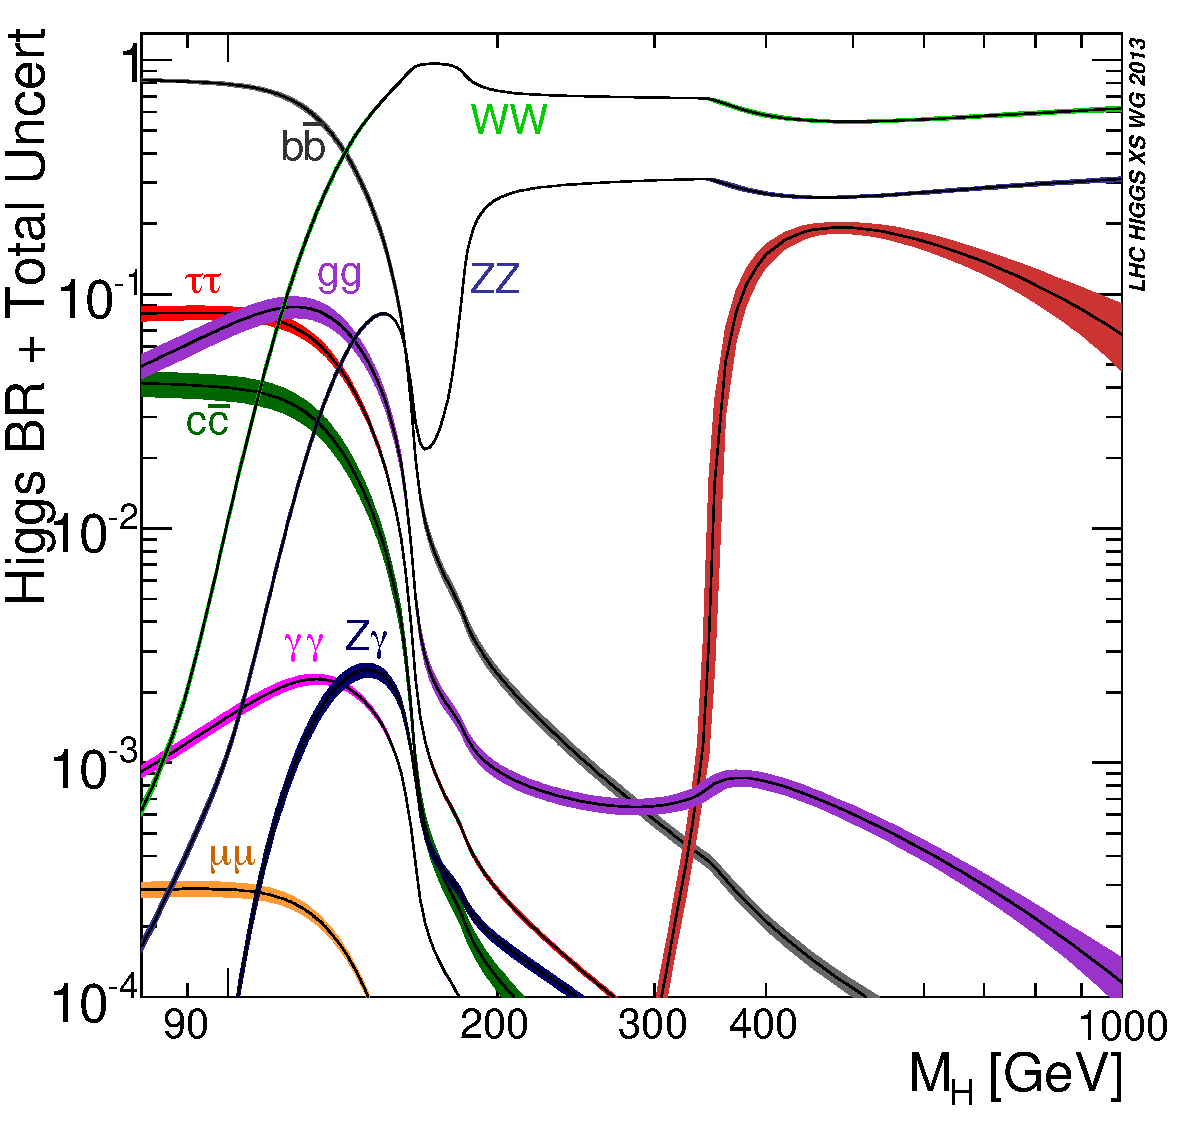
\includegraphics[width=0.6\textwidth]{plots/theory/Higgs_BR.pdf}
\caption[Higgs boson branching ratios in the SM for a range of Higgs boson
masses.]{Higgs boson branching ratios in the SM for a range of Higgs boson
masses $m_{\PH}$ \cite{Heinemeyer:2013tqa}. Whilst the $\PW\PW$ and $\PZ\PZ$
decay modes dominate at higher Higgs masses, at lower masses a wide range of
different final states is possible.}
\label{fig:SMHiggsBRs}
\end{figure}

On 4 July 2012 the ATLAS and CMS Collaborations announced the discovery of a new
boson with a mass around $125\,\GeV$ \cite{CMSobservation125,ATLASobservation125}. 
Both experiments analysed approximately $5\,\invfb$ of data collected at 
$\sqrt{s}=7\,\TeV$ and $5$--$6\,\invfb$ at $\sqrt{s}=8\,\TeV$. The discovery was
made predominantly using the $\PZ\PZ$ and $\Pphoton\Pphoton$ decay modes with a
combined excess of events in data yielding a $5\sigma$ deviation from the
background-only expectation.

Run 1 of the LHC was completed in early 2013, increasing the dataset to
$\approx20\,\invfb$ at $8~\TeV$. The increased dataset allows access to the less
sensitive decay modes. The most recent combination of CMS Higgs results yields a
best fit mass of
$125.02^{+0.26}_{-0.27}(\text{stat})^{+0.14}_{-0.15}(\text{syst})~\GeV$ and a
signal strength relative to the \ac{SM} expectation of
$1.00\pm1.09(\text{stat})^{+0.08}_{-0.07}(\text{theo})\pm0.01(\text{syst})$,
combining results from the $\Pphoton\Pphoton$, $\PWp\PWm$, $\PZ\PZ$,
$\Pqb\Paqb$, $\Pgtp\Pgtm$ and $\APmuon\Pmuon$ final states, as well as 
searches for the $\Pqt\Pqt\PH$ production mode and searches for an invisible
Higgs \cite{CMScomb}. Within the combination is a study of the compatibility of
the couplings in each decay mode with the \ac{SM}. 
These channels all show consistency with the \ac{SM}
predictions for a $125~\GeV$ Higgs boson. Other analyses from ATLAS have
studied the production rates and couplings in various channels
~\cite{Aad:2014eva,Aad:2014lwa,Aad:2015vsa}, and results from both ATLAS and CMS study 
the spin-parity quantum
numbers~\cite{Chatrchyan:2013mxa,Chatrchyan:2013iaa,Aad:2013xqa} and limits on
the decay width ~\cite{Khachatryan:2014iha} and invisible branching
fraction~\cite{Aad:2014iia,Chatrchyan:2014tja}. No significant deviations from \ac{SM}
predictions have been found to date in any of these results.

Future studies will further test the compatibility of the observed boson with
the \ac{SM} Higgs, including discovery and precision measurements in the
channels which are less sensitive and require more data. 
The most recent CMS results for the search for the Higgs boson in the $\HToTauTau$
decay channel, corresponding to the complete Run 1 dataset and as included in
the most recent combination, are reported in chapter~\ref{chap:htt-sm}.

\section{Higgs Physics Beyond the Standard Model}
\label{sec:BSM}

\subsection{Motivation for theories beyond the Standard Model}
\label{sec:hierarchyproblem}

Despite its successes, the \ac{SM} is known to have some shortcomings. As a
theory, it does not predict a candidate to account for the large fraction of
non-radiating, non-baryonic dark matter in the universe. It also does not
predict the non-zero neutrino masses which are inferred from experimental
results in neutrino oscillations \cite{PDG}. As a theory it also suffers from a
shortcoming in that the weak and strong coupling constants associated with the
$SU(3)_{C} \times SU(2)_{L} \times U(1)_{Y}$ gauge group do not intersect at a
high energy scale, as would be hoped for in a unified theory. It also does not
incorporate gravity. Finally, one shortcoming is of particular relevance 
in the Higgs sector, and is known as the Hierarchy Problem.

It is generally accepted that the \ac{SM} is an effective theory up to some
energy scale $\Lambda$ where the effect of new physics becomes important. 
The Higgs mass at tree level is given by $\sqrt{2}\mu_{SM}$. Radiative
corrections adjust the mass as:
\begin{equation}
m_{\PH_{SM}}^{2} = 2\mu_{SM}^{2} - \Delta m_{\PH}^{2}. 
\end{equation}
It can be shown that the size of the correction, $\Delta m_{\PH}^{2}$, is
quadratically dependent on $\Lambda$ \cite{Carena:2002es}:
\begin{equation}
\Delta m_{\PH}^{2} \sim \mathcal{O}(\Lambda^{2}).
\end{equation}
The scale $\Lambda$ can be as high as the Planck scale, where gravitational
interactions become significant \cite{Griffiths:2008nx}. For a $\Lambda$ at the Planck scale then
$\Delta m_{\PH}^{2}$ is some 30 orders of magnitude larger than 
$m_{\PH_{SM}}^{2}$ for $m_{\PH_{SM}}<1~\TeV$. This means that the bare Higgs
boson mass requires extreme fine tuning of the bare mass term $2\mu_{SM}^{2}$ to
allow cancellation. Figure \ref{fig:HiggsMassLoops} indicates the radiative
corrections to the Higgs mass resulting from a fermion and a boson loop.

\begin{figure}[htbp]
\subfloat[]{
   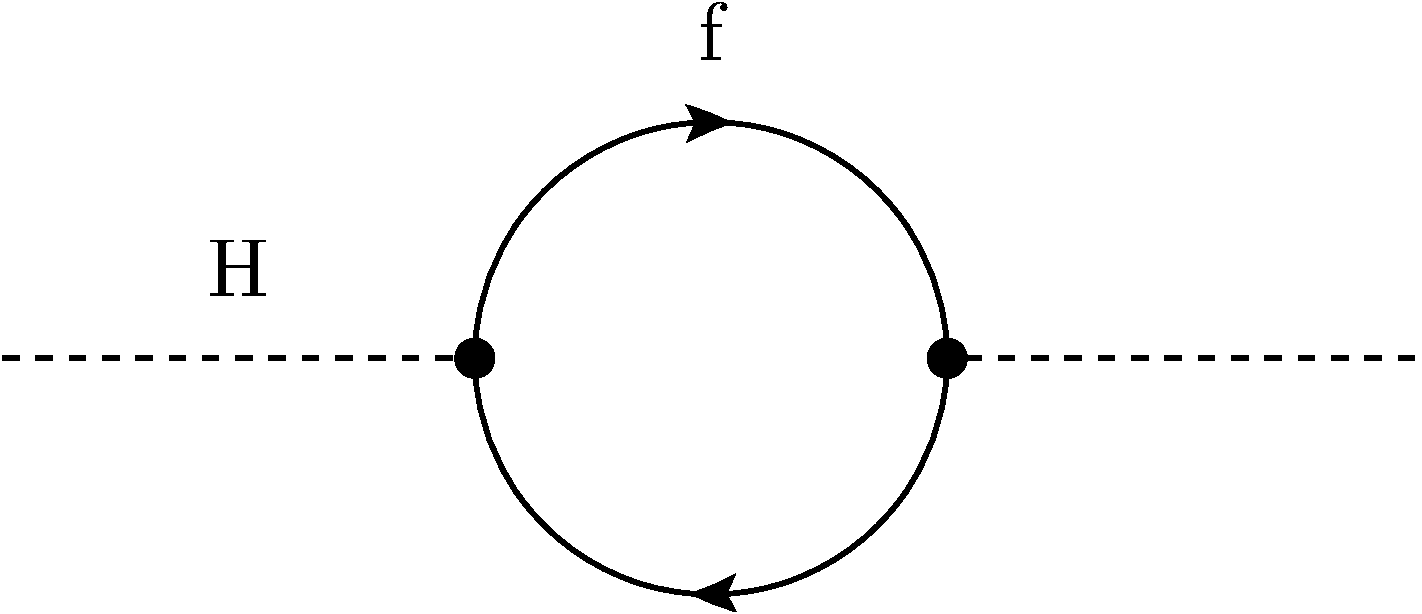
\includegraphics[width=0.48\textwidth]{plots/theory/HiggsMass_fermionLoop.pdf}}
\subfloat[]{
   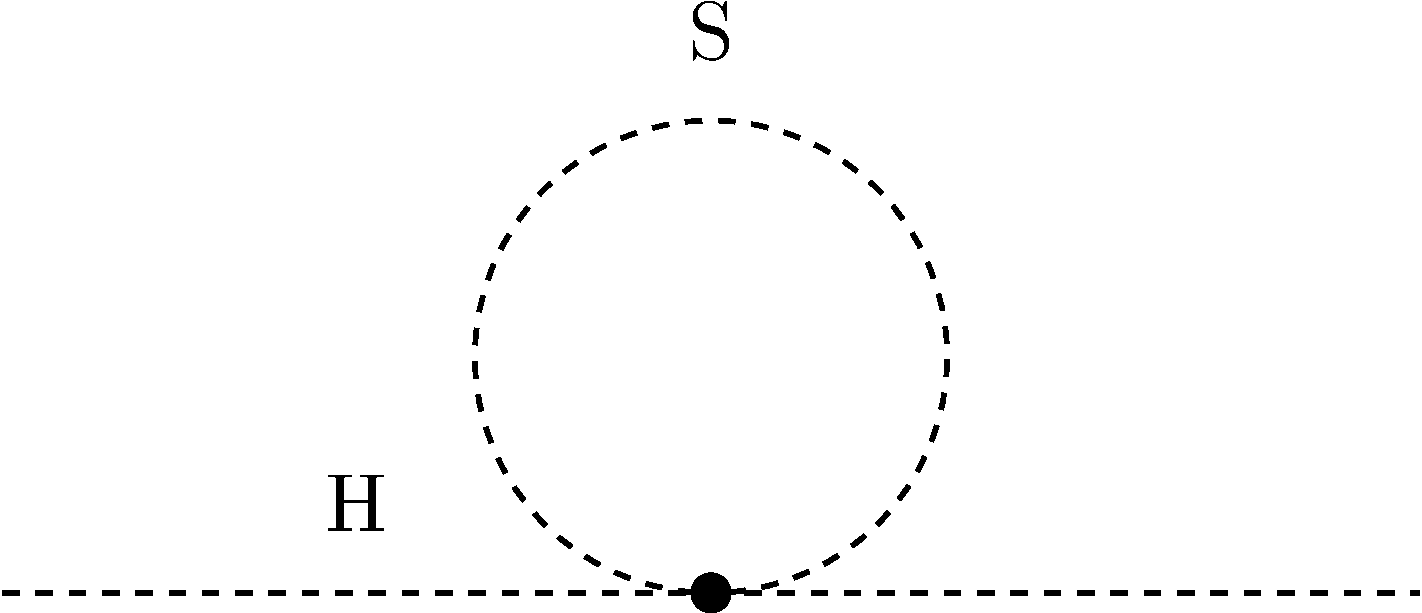
\includegraphics[width=0.48\textwidth]{plots/theory/HiggsMass_bosonLoop.pdf}}
\caption{Feynman diagrams illustrating the one-loop radiative corrections to the Higgs
mass for a fermion, $f$, and scalar boson, $S$.}
\label{fig:HiggsMassLoops}
\end{figure}

Many \ac{BSM} theories are proposed which provide solutions to this Hierarchy
problem. One of the most popular is supersymmetry (SUSY). In SUSY, a new
symmetry between fermions and bosons is introduced \cite{Martin:1997ns}. This
can be used to solve the issue with the Higgs mass correction by exploiting the
fact that the bosonic and fermionic loop contributions illustrated in figure
\ref{fig:HiggsMassLoops} contribute with opposite signs. Thus the symmetry
between bosons and fermions permits the cancellation of $\Delta m_{\PH}^{2}$
terms. In SUSY models, each \ac{SM} fermion has a boson superpartner and each
\ac{SM} boson has a fermion superpartner. If SUSY is an unbroken symmetry then
the superpartners have exactly the same mass as their \ac{SM} partner. Since
none of these superpartner particles have been observed in nature, SUSY must be
an unbroken symmetry in which the superpartner masses are larger than the
\ac{SM} masses. The necessity to avoid further fine tuning means the scale of
SUSY cannot be much larger than $\mathcal{O}(1\,\TeV)$. An additional motivation
for SUSY is the fact that the lightest SUSY particles, if stable, could provide
candidates for dark matter. Also the behaviour of the running coupling
constants is modified such that all three intersect at
$\mathcal{O}(10^{16}\,\GeV)$ \cite{Amaldi:1991cn}.

\subsection{The Higgs sector in the MSSM}
\label{sec:mssmhiggs}

The simplest addition of SUSY to the \ac{SM} results in the \ac{MSSM}. The
\ac{MSSM} is an extension to the \ac{SM} which minimises the numbers of
additional fields and interactions while preserving R-parity \cite{Dimopoulos:1981zb}. R-parity
is an operator with eigenvalues of 1 for \ac{SM} particles and -1 for
superparners. It is required to be conserved in order to explain the stability
of the proton. In order to generate the appropriate mass terms for the up-type 
and down-type fermions, two complex scalar weak isospin doublet fields
$\phi_{\Pqu}$ and $\phi_{\Pqd}$ are added:
\begin{equation}
\phi_{\Pqu} = \begin{pmatrix}\phi_{\Pqu}^{+} \\ \phi_{\Pqu}^{0} \end{pmatrix}, \quad
\phi_{\Pqd} = \begin{pmatrix}\phi_{\Pqd}^{0} \\ \phi_{\Pqd}^{-} \end{pmatrix}. 
\end{equation}
This results in an \ac{MSSM} Lagrangian with potential terms as:
\begin{equation}
V=\mu(\phi_{\Pqu}^{+}\phi_{\Pqd}^{-} - \phi_{\Pqu}^{0}\phi_{\Pqd}^{0}),
\end{equation}
where $\mu$ is the \ac{MSSM} equivalent of the \ac{SM} Higgs mass parameter
$\mu_{SM}$. This potential provides spontaneous symmetry breaking as in the
\ac{SM} case yielding VEVs parameterised by:
\begin{equation}
\bra{0}\phi_{\Pqu}\ket{0} = \begin{pmatrix} 0 \\ v_{\Pqu}  \end{pmatrix}, \quad
\bra{0}\phi_{\Pqd}\ket{0} = \begin{pmatrix} v_{\Pqd} \\ 0 \end{pmatrix},
\end{equation}
which are related to the \ac{SM} value and hence $m_{\PW}$ by: 
\begin{equation}
v^{2} = v_{\Pqu}^{2} +  v_{\Pqd}^{2} =  \frac{2m_{\PW}^{2}}{g},
\end{equation}
Thus in the \ac{MSSM}, the
phenomenology is conveniently described in terms of the ratio of the VEVs,
$\tan\beta = v_{u}/v_{d}$, which is not directly predicted by the model.
Of the eight initial degrees of freedom, three become longitudinal states of the
$\PW^{\pm}$ and $\PZ$ bosons which leaves five massive Higgs fields. These
result in five physical Higgs bosons; a neutral pseudoscalar $\PA$, two neutral
scalars $\Ph,\PH$ and two charged scalars $\PH^{\pm}$. These bosons are defined
by the mixing of $\phi_{\Pqu}$ and $\phi_{\Pqd}$, parameterised by a mixing
angle $\alpha$ in addition to $\beta$:
%Check this - typo in Mike's thesis?
\begin{equation}
\PA = \sqrt{2}(\text{Im}(\phi_{\Pqu}^{0})\cos\beta +
\text{Im}(\phi_{\Pqd}^{0})\sin\beta), \\ 
\begin{pmatrix} h \\ H \end{pmatrix} = \sqrt{2} 
\begin{pmatrix} \cos\alpha & -\sin\alpha \\ \sin\alpha & \cos\alpha \end{pmatrix}
\begin{pmatrix} \text{Re}(\phi_{\Pqu}^{0}) - v_{\Pqu} \\ \text{Re}(\phi_{\Pqd}^{0}) -
v_{\Pqd}\end{pmatrix}, \\
\PH^{+} = \phi_{\Pqu}^{+} \cos \beta + \phi_{\Pqd}^{-\dagger} \sin \beta,\\
\PH^{-} = \phi_{\Pqu}^{+\dagger} \cos \beta + \phi_{\Pqd}^{-} \sin \beta.
\end{equation}
The self interactions of the scalar fields are not independent parameters in the
\ac{MSSM} and can be expressed in terms of $g$ and $g'$. As a result, the masses
and couplings of the \ac{MSSM} Higgs bosons can be determined at tree level by
two free parameters: $\tan\beta$ and the mass of one of the Higgs bosons,
conventionally chosen to the the mass of the pseudoscalar, $m_{\PA}$. The masses
of the other Higgs bosons can then be expressed as:
\begin{equation}
m_{\Ph}^{2} = \frac{1}{2} \left( m_{\PA}^{2} + m_{\PZ}^{2} - \sqrt{(m_{\PA}^{2} +
m_{\PZ}^{2})^{2} - 4m_{\PZ}^{2}m_{\PA}^{2}\cos{2\beta}^{2} }\right) ,
\label{eq:mh}\\
m_{\PH}^{2} = \frac{1}{2} \left( m_{\PA}^{2} + m_{\PZ}^{2} + \sqrt{(m_{\PA}^{2} +
m_{\PZ}^{2})^{2} - 4m_{\PZ}^{2}m_{\PA}^{2}\cos{2\beta}^{2} }\right) , \\
m_{\PH^{\pm}} = m_{\PA}^{2} + m_{\PW}^{2},
\end{equation}
where $m_{\Ph}$, $m_{\PH}$ and $m_{\PH^{\pm}}$ are the masses of the $\Ph$,
$\PH$ and $\PH^{\pm}$ bosons respectively. This yields a constraint on $\alpha$:
\begin{equation}
\cos^{2}(\beta-\alpha) = \frac{m_{\Ph}^{2}(m_{\PZ}^{2} -
m_{\Ph}^{2})}{m_{\PA}^{2}(m_{\PH}^{2} - m_{\Ph}^{2}) }.
\end{equation}
Equation \ref{eq:mh} yields an upper bound on $m_{\Ph}$:
\begin{equation}
m_{\Ph} \leq m_{\PZ} |\cos{2\beta}|. 
\end{equation}

This means that at tree level, the mass of the lightest scalar Higgs cannot
exceed that of the $\PZ$ boson ($91.2~\GeV$). However, the tree level masses and
couplings are modified by higher order corrections. The dominant effect is from
incomplete cancellation of the top and stop (the superpartner of the top) loops.
These corrections, as illustrated in figure \ref{fig:HiggsMassLoops}, do not
completely cancel in the case that SUSY is broken. Hence the size of the
corrections are strongly dependent on the top and stop masses, where the stop
mass depends on $\mu$ and the parameters describing SUSY breaking. The upper
bound of $m_{\Ph}$ is increased by these radiative corrections and is maximised
for large $m_{\PA}$ ($\gg m_{\PZ}$) and $\tan\beta$ ($\gg1$). The maximum value of
$m_{\Ph}$ for a particular choice of $m_{\PA}$ and $\tan\beta$ is denoted
$m_{\Ph}^{\text{max}}$. If the scale of SUSY breaking, $M_{\text{SUSY}}$ is
chosen to be $1~\TeV$, $m_{\Ph}^{\text{max}} \approx 135~\GeV$.

\subsection{Searching for a neutral MSSM Higgs boson}
\label{sec:LHCMSSMHiggs}

It is important that the phenomenology of Higgs bosons, including the higher
order corrections, is understood in order to define the masses of the neutral
Higgs bosons and hence optimise an experimental search for them. This is
complicated by the number of SUSY breaking parameters in the \ac{MSSM}. Hence it
is conventional to study particular benchmark scenarios where the SUSY breaking
parameters and $\mu$ are fixed to a choice of values and only $m_{\PA}$ and
$\tan\beta$ are varied \cite{Carena:2002es}. One such scenario is the $m_{\Ph}^{\text{max}}$ scenario
in which $m_{\Ph}=m_{\Ph}^{\text{max}}$ for high $m_{\PA}$ and $\tan\beta$
values, using the choice $M_{\text{SUSY}} = 1~\TeV$ and $\mu = \pm 200~\GeV$.
Other alternative benchmark scenarios are discussed in 
section~\ref{sec:mssmbenchmarks}. 

Figure \ref{fig:mhmaxmasses} indicates the
masses of each of the Higgs bosons in the $m_{h}^{\text{max}}$ scenario
for $\tan\beta=3$ and $\tan\beta=30$ as a function of the mass of the
pseudoscalar $m_{\PA}$. Two different regimes of the $m_{\Ph}^{\text{max}}$
scenario can be considered, in which one of the neutral scalars is approximately
degenerate in mass with the pseudoscalar and has similar couplings. 
At large $\tan\beta$ and for $m_{\PA} \ll m_{\Ph}^{\text{max}}$, $m_{\PA}
\approx m_{\Ph}$ and the couplings of the $\PA$ and $\Ph$ are very similar. The
couplings of the $\PA$ and $\Ph$ bosons to down-type fermions 
are enhanced by a factor $\sim \tan\beta$ relative to the \ac{SM} value, with
negligible couplings to vector bosons. The scalar $\PH$ has couplings
close to those in the \ac{SM}. In the limit where $m_{\PA} \gg
m_{\Ph}^{\text{max}}$, 
$m_{\PA} \approx m_{\PH}$ and the couplings of the $\PA$ and $\PH$ are
very similar. The couplings of the $\PA$ and $\PH$ bosons to down-type fermions 
are enhanced by a factor $\sim \tan\beta$ relative to the \ac{SM} value, 
with neglible couplings to vector bosons. The scalar $\Ph$ has couplings
close to those in the \ac{SM}. 

\begin{figure}[htbp]
   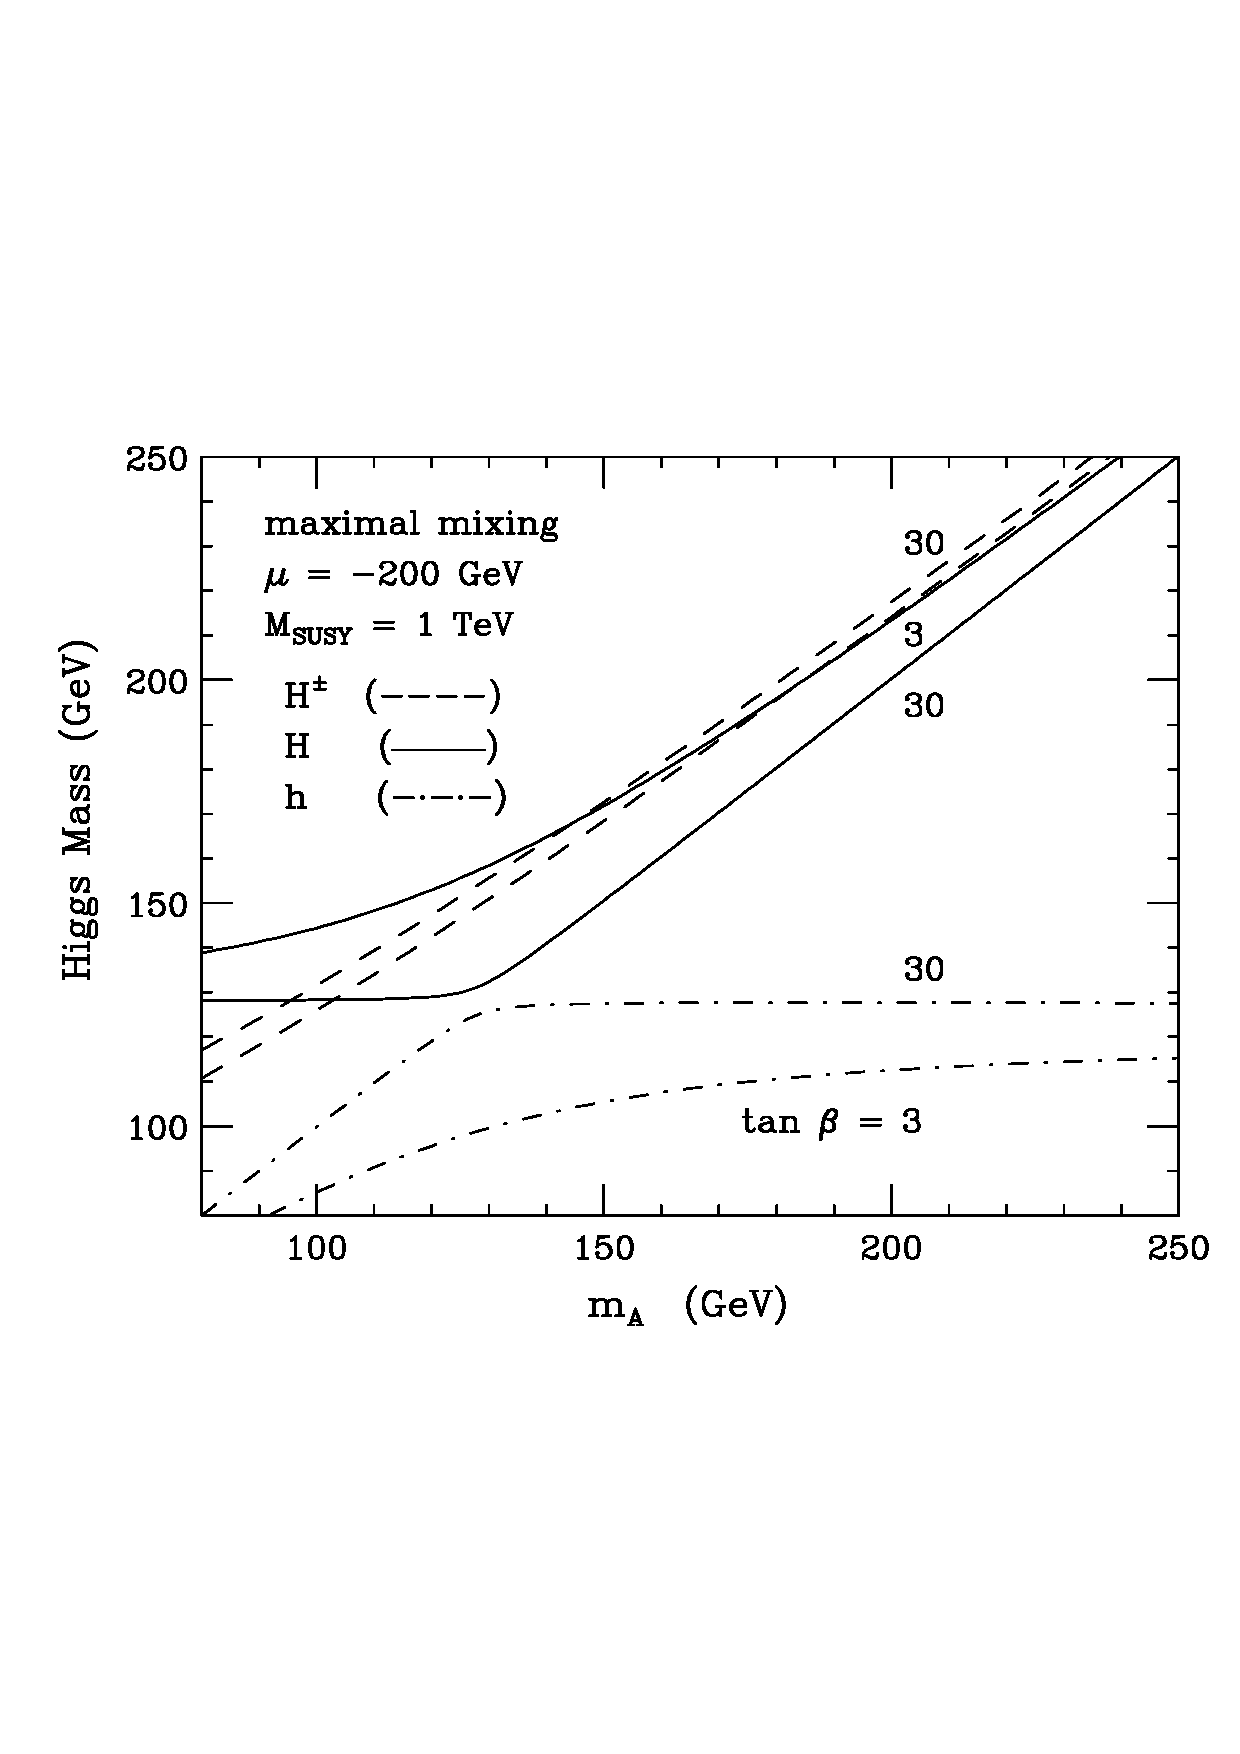
\includegraphics[width=0.7\textwidth]{plots/theory/mssm_masses_mhmax.pdf}
\caption[Masses of the $\Ph$, $\PH$ and $\PH^{\pm}$ bosons in the
$m_{\Ph}^{\text{max}}$ scenario as a function of $m_{\PA}$.]{Masses of the $\Ph$, $\PH$ and $\PH^{\pm}$ bosons in the
$m_{\Ph}^{\text{max}}$ scenario as a function of $m_{\PA}$. Values are shown for
$\tan\beta=3$ and $\tan\beta=30$ \cite{Carena:2002es}.}
\label{fig:mhmaxmasses}
\end{figure}

The effect of enhanced couplings to down-type fermions is illustrated by the
branching ratios of the $\PA$, shown in figure \ref{fig:mhmaxBRs} for $\tan\beta$
values of 10 and 50. It can be seen that the $\Pgt\Pgt$ decay mode has a large
branching ratio for a large range of $m_{\PA}$ and $\tan\beta$ points. This
motivates searches for the \ac{MSSM} Higgs bosons in the final state of $\Pgt\Pgt$. 
Chapter \ref{chap:htt-mssm} discusses the most recent results 
from direct searches for neutral \ac{MSSM} Higgs bosons using the $\Pgt\Pgt$
final state with the CMS detector.

\begin{figure}[htbp]
\subfloat[]{
   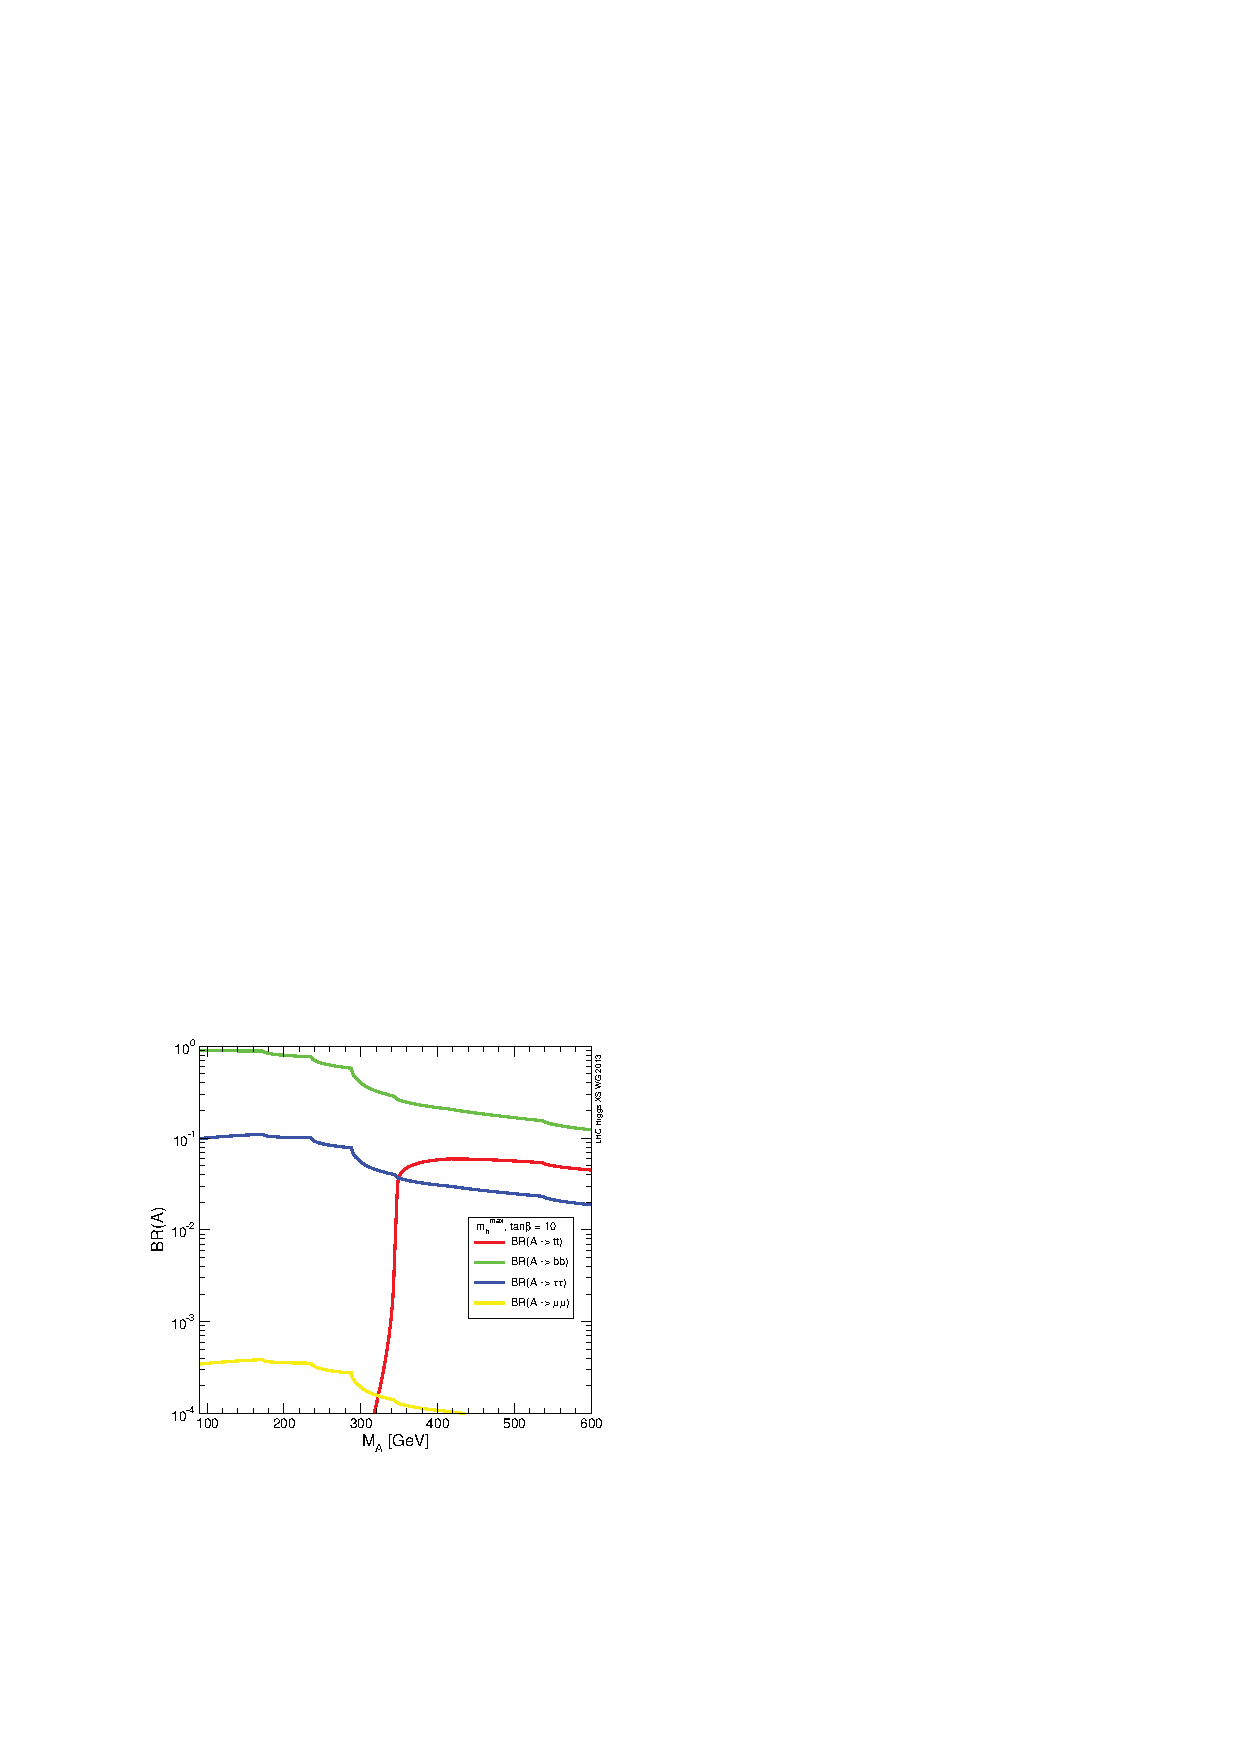
\includegraphics[width=0.5\textwidth]{plots/theory/BR_A_tanb10_mhmax.pdf}}
\subfloat[]{
   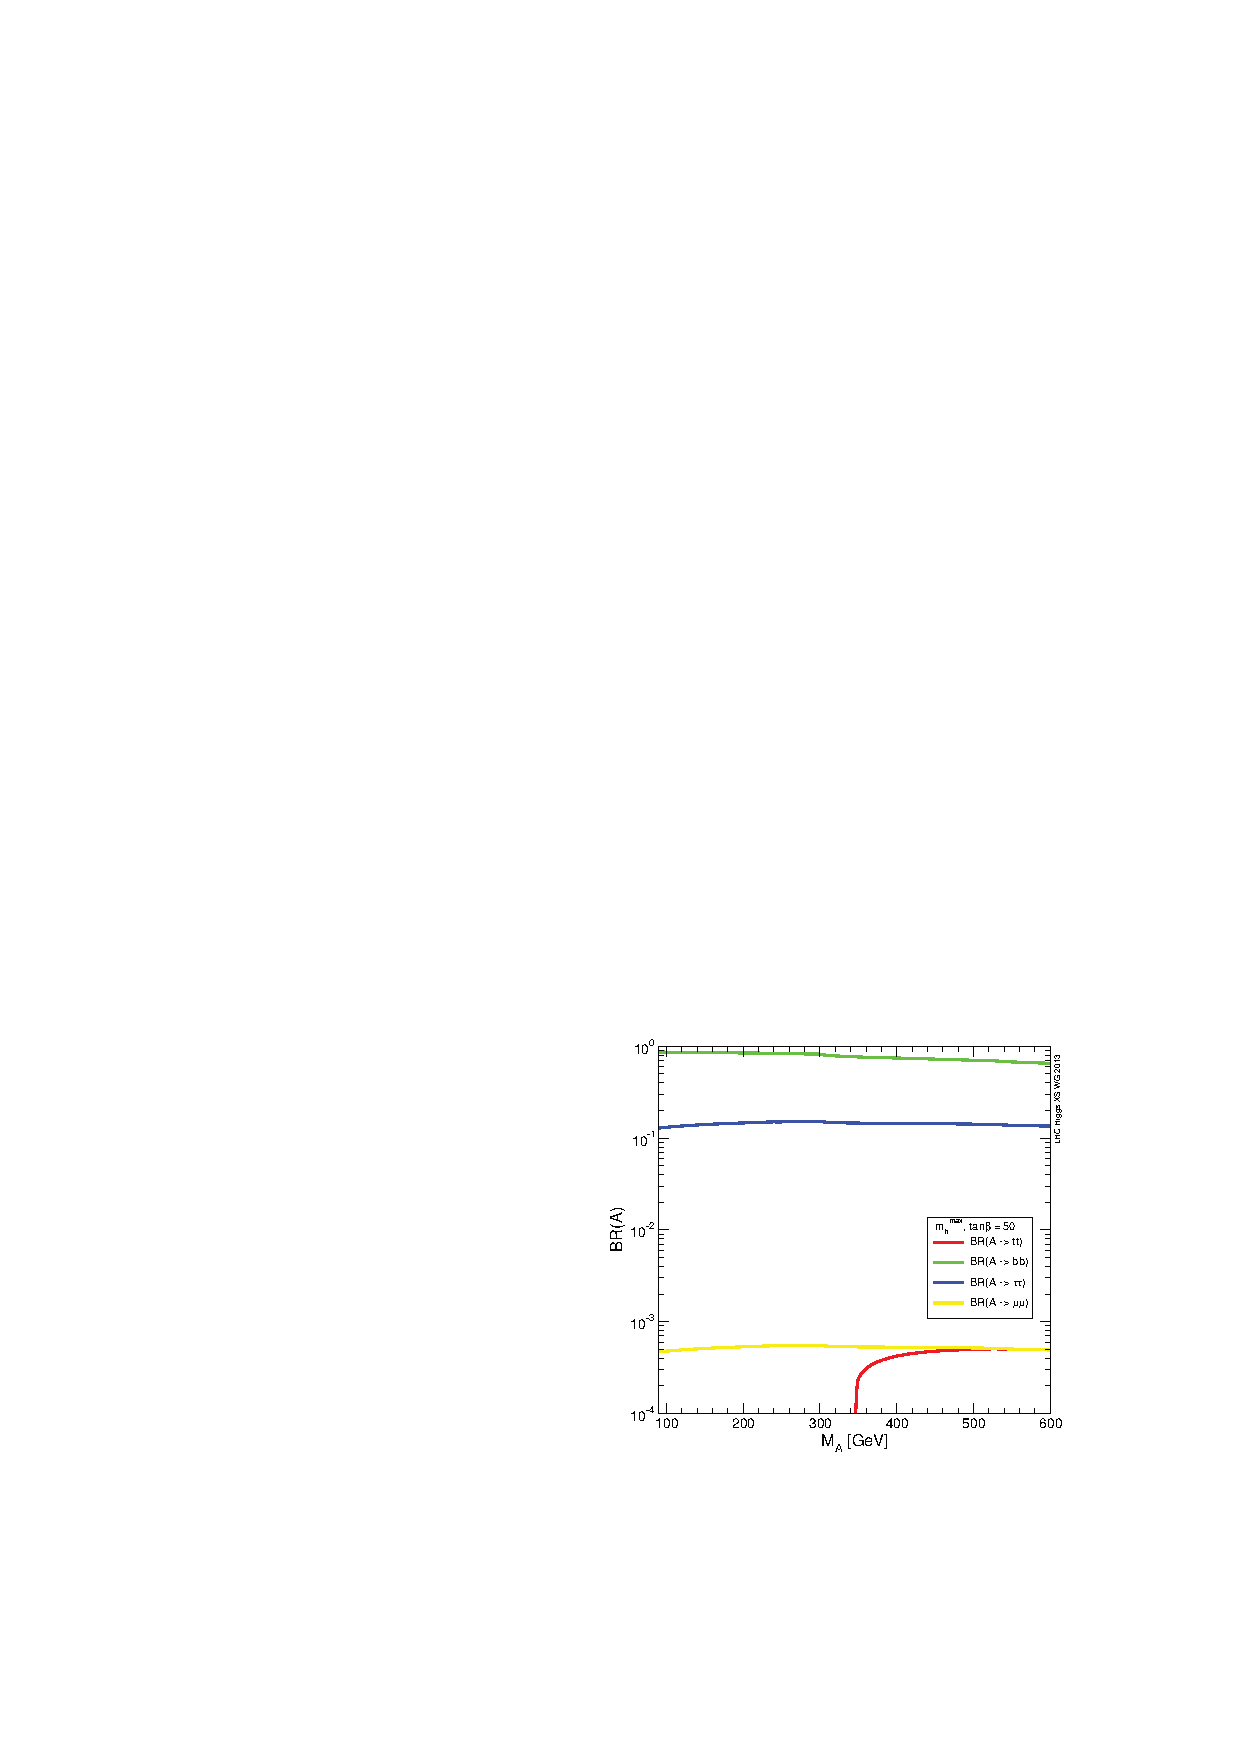
\includegraphics[width=0.5\textwidth]{plots/theory/BR_A_tanb50_mhmax.pdf}}
\caption[Branching ratios of the pseudoscalar Higgs boson $\PA$ in the
$m_{\Ph}^{\text{max}}$ scenario.]{Branching ratios of the pseudoscalar Higgs boson $\PA$ in the
$m_{\Ph}^{\text{max}}$ scenario for $\tan\beta=10$ (left) and $\tan\beta=50$
(right) \cite{Heinemeyer:2013tqa}.}
\label{fig:mhmaxBRs}
\end{figure}

Analogously to the \ac{SM} Higgs production, the dominant production mode at
small $\tan\beta$ is the gluon-gluon fusion process, denoted
$\Pgluon\Pgluon\to\Pphi$, where $\Pphi$ denotes any of the three neutral Higgs
bosons, $\Pphi=\PH,\PA,\Ph$. As in the \ac{SM} case the gluon fusion process
proceeds via a quark loop, which at low $\tan\beta$ is dominated by top quarks
but at high $\tan\beta$ the $\Pqb$-quark loops dominate due to enhanced couplings to
down-type fermions. At large $\tan\beta$, the dominant production mechanism is
Higgs radiation by $\Pqb$-quarks, denoted $\Pgluon\Pgluon\to\Pqb\Pqb\Pphi$.
Example tree level Feynman diagrams illustrating these two production processes
are shown in figure~\ref{fig:mssmfeynman}. The cross-sections for each of these 
production processes are shown in
figure~\ref{fig:mhmaxXSs} for $\sqrt{s}=8~\TeV$, evaluated in the $m_{\Ph}^{\text{max}}$
scenario.

\begin{figure}[htbp]
\subfloat[]{
   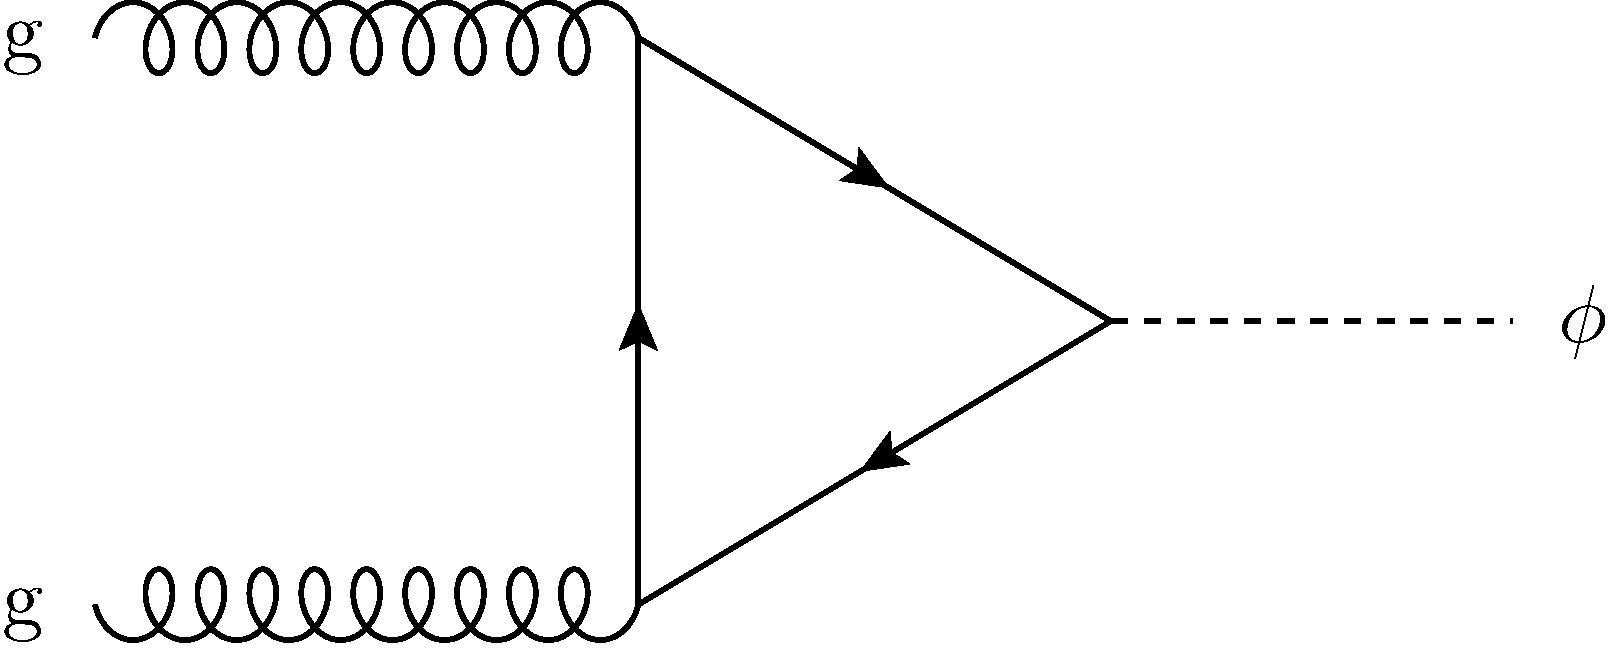
\includegraphics[width=0.55\textwidth]{plots/theory/feynman_mssm_ggH.pdf}}
\subfloat[]{
   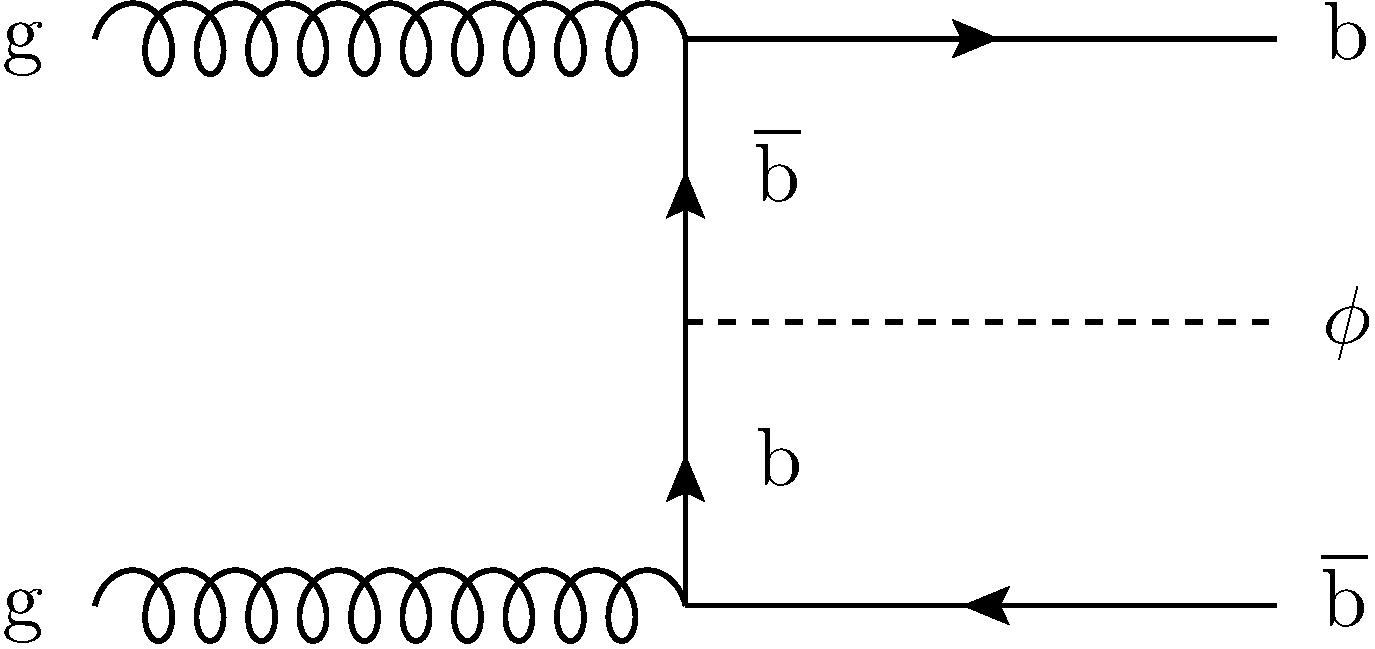
\includegraphics[width=0.45\textwidth]{plots/theory/feynman_mssm_bbH.pdf}}
\caption[Feynman diagrams illustrating example tree level production of neutral
Higgs bosons in the MSSM.]{Feynman diagrams illustrating example tree level production for the
gluon-fusion process (left) or b-assocated production process (right). The
particle $\Pphi$ indicates any one of the three neutral Higgs bosons, $\Ph$,
$\PH$ or $\PA$.}
\label{fig:mssmfeynman}
\end{figure}

\begin{figure}[htbp]
\subfloat[]{
   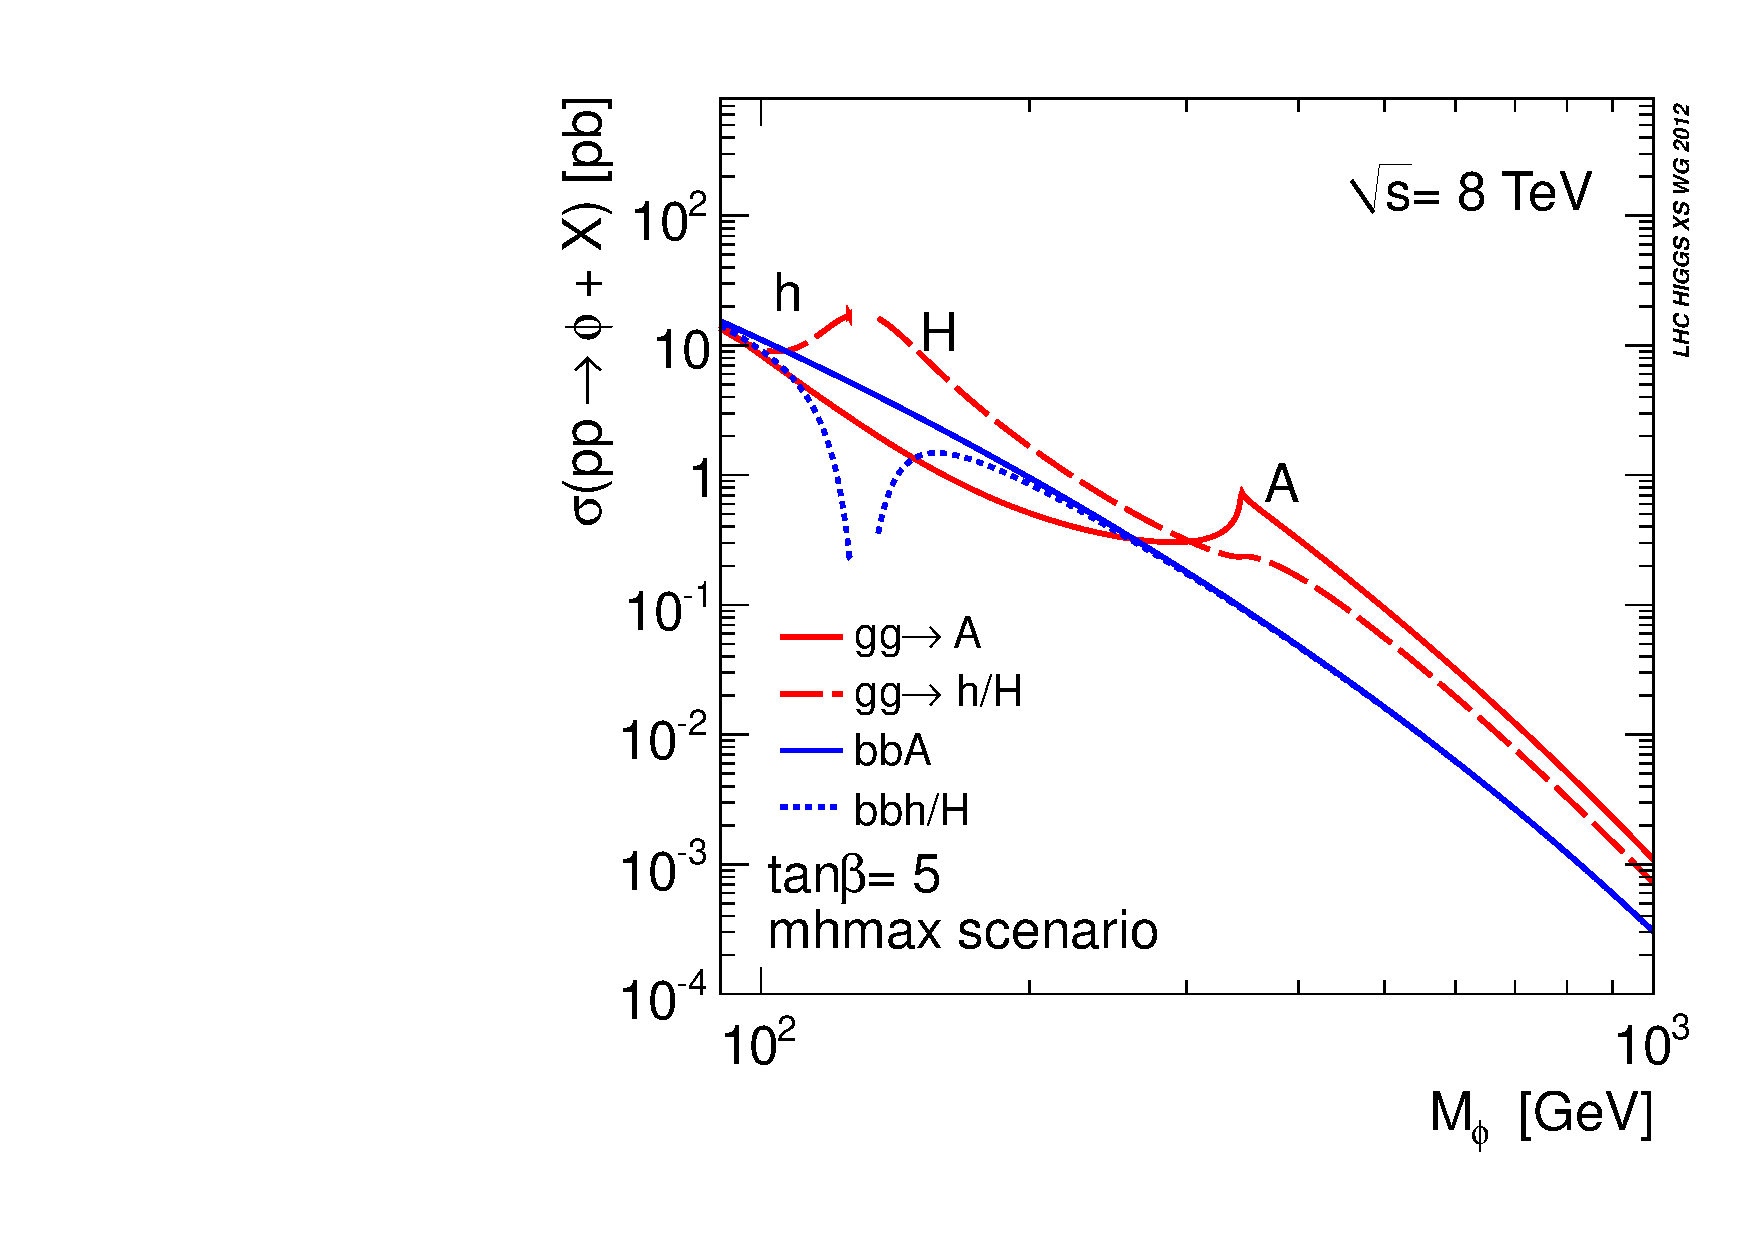
\includegraphics[width=0.5\textwidth]{plots/theory/YR3HXS_XSectSummary_mhmax8TeV_tanbeta5.pdf}}
\subfloat[]{
   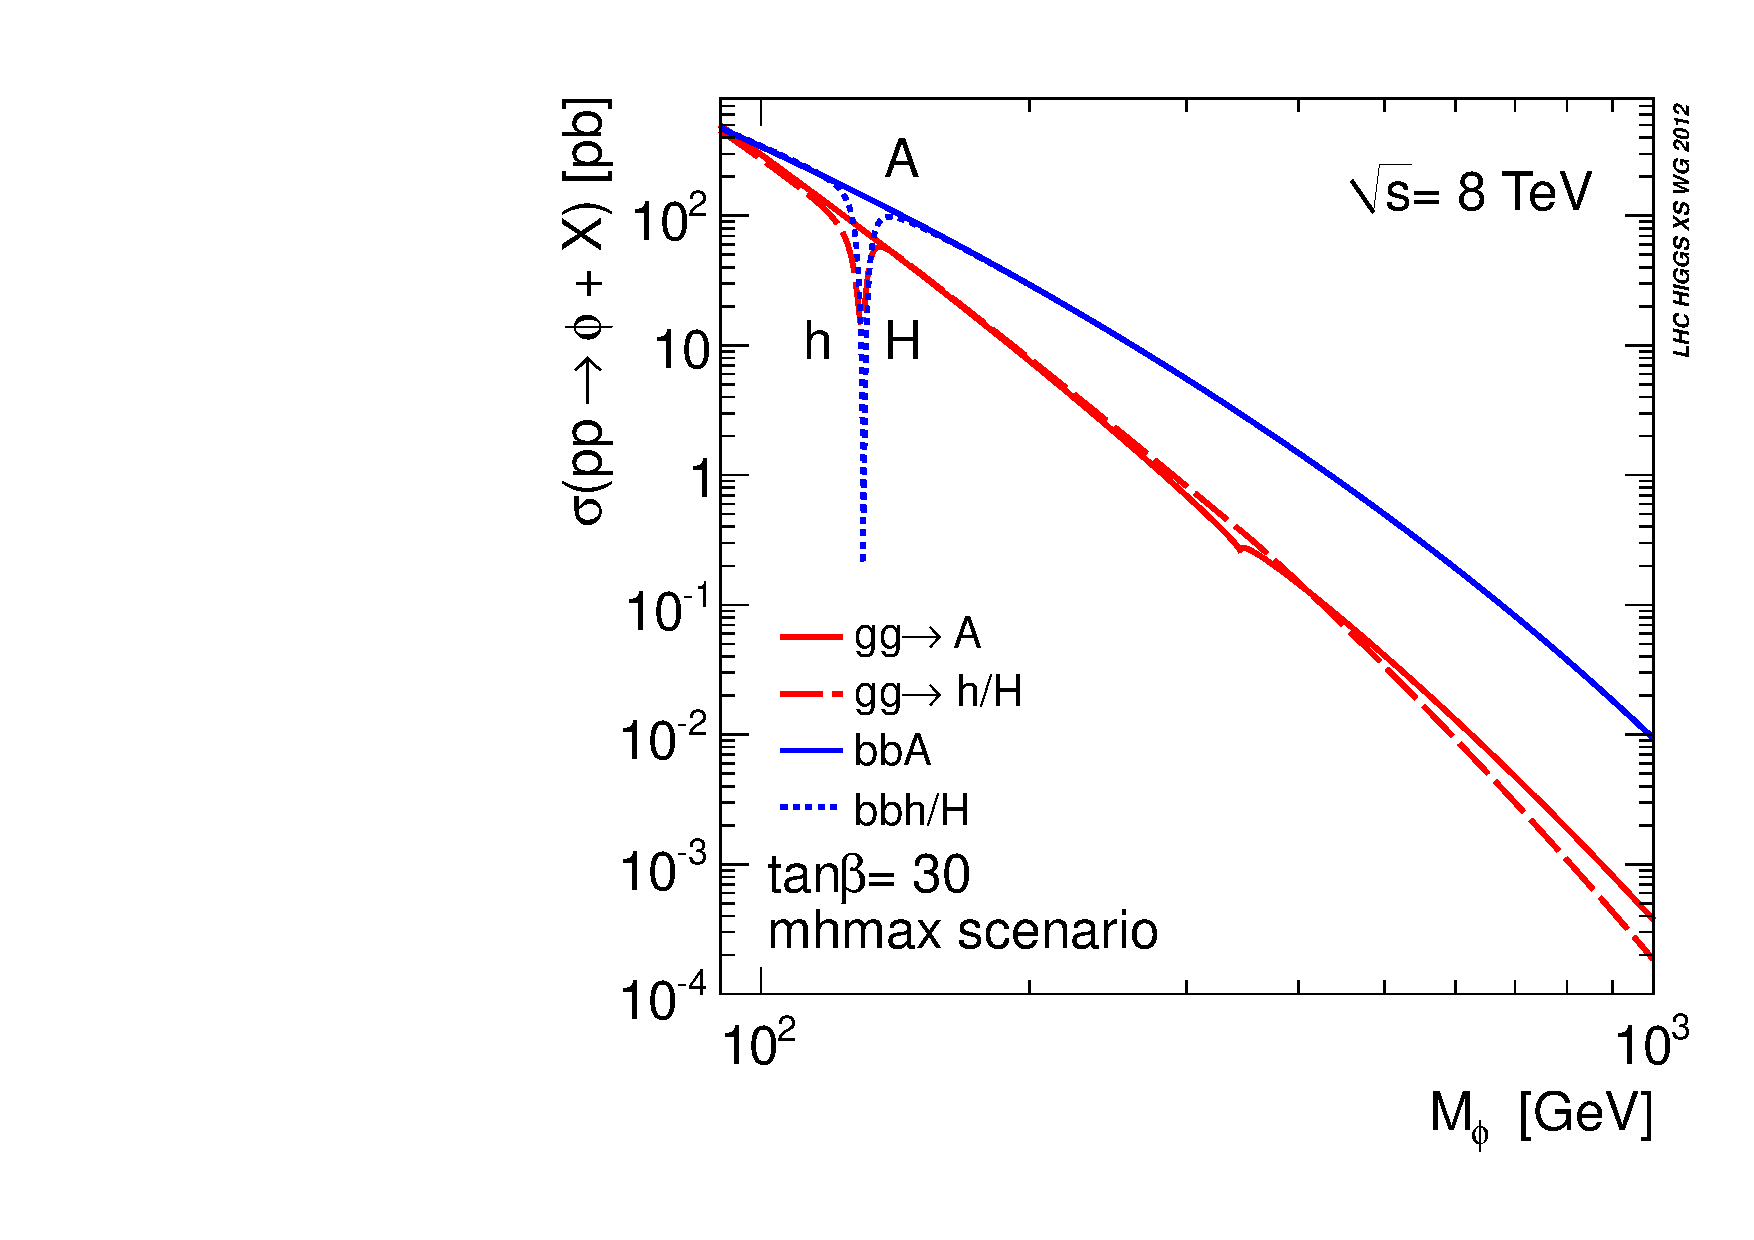
\includegraphics[width=0.5\textwidth]{plots/theory/YR3HXS_XSectSummary_mhmax8TeV_tanbeta30.pdf}}
\caption[Cross-sections for the production of neutral MSSM Higgs bosons in the 
$m_{\Ph}^{\text{max}}$ scenario.]{Cross-sections for the production of neutral MSSM Higgs bosons in the 
$m_{\Ph}^{\text{max}}$ scenario for $\tan\beta=5$ (left) and $\tan\beta=30$
(right) \cite{Heinemeyer:2013tqa}.}
\label{fig:mhmaxXSs}
\end{figure}

Previous searches for neutral \ac{MSSM} Higgs bosons were conducted at LEP, with
interpretation in the $m_{\Ph}^{max}$ scenario \cite{Schael:2006cr}.
The results were negative and yielded limits $m_{\PA} > 93.4~\GeV$ at $95\%$ CL.  
Results from the Tevatron \cite{Benjamin:2010xb} provide complementary exclusion 
limits at high $\tan\beta$, considering masses up to $m_{\PA}=200~\GeV$. The
higher centre of mass energy of the LHC provides access to $m_{\PA}$ values as
high as $1~\TeV$. The most recent results from the LHC exclude large regions of
previously unreachable phase space in the $m_{h}^{\text{max}}$ scenario
\cite{Aad:2014vgg,HIG-13-021}. The results discussed in
chapter~\ref{chap:htt-mssm} follow those in \cite{HIG-13-021}.

\section{MSSM Models incorporating the LHC Higgs}
\label{sec:mssmbenchmarks}

With the discovery of a 125$~\GeV$ Higgs-like particle at the LHC, the number of
possible \ac{MSSM} scenarios is reduced to those which can incorporate this boson
with its measured properties. This section details some possible \ac{MSSM} scenarios
which can incorporate this 125$~\GeV$ boson, whilst also exhibiting interesting
phenomenology motivated by experimental measurements. In particular the
scenarios must fulfil the condition $m_{\PH} = 125 \pm 3~\GeV$ over a wide range
of parameter space, and satisfy the boundaries set by previous searches at LEP,
the Tevatron and the LHC. The $3~\GeV$ uncertainty on the Higgs mass is
dominated by theoretical uncertainties in the MSSM models. All of the scenarios 
considered are defined without allowing CP violation. The scenarios follow those
described in~\cite{MSSMScenarios}, with some small modifications. More detail
can be found in~\cite{HIG-13-021}, where these scenarios are discussed in the context
of the MSSM $\Pphi \to \Pgt\Pgt$ analysis. 

As described previously, at tree level the masses of the five Higgs bosons are
defined by $m_{\PA}$ and $\tan\beta$. These masses are adjusted via radiative
corrections, necessary to produce a Higgs with mass consistent with $125~\GeV$.
The parameters of interest in these radiative corrections are as follows:

\begin{itemize}
\item The mass of the top quark, $m_{\Pqt}$.
\item The mass of the bottom quark, $m_{\Pqb}$.
\item The mass of the 3rd generation squarks: stops and sbottoms, given by
$M_{\text{SUSY}}$.
\item The higgsino mass parameter, $\mu$.
\item The mass of the 3rd generation sleptons: the staus, given by
$M_{\PSlepton_{3}}$.
\item The $U(1)$ gaugino mass parameter, $M_{1}$.
\item The $SU(2)$ gaugino mass parameter, $M_{2}$.
\item The trilinear couplings of the stops, sbottoms and staus, $A_{\Pqt}$,
$A_{\Pqb}$ and $A_{\Pgt}$.
\item The mixing parameters of the stops, sbottoms and staus, $X_{\Pqt}$,
$X_{\Pqb}$ and $X_{\Pgt}$.
\end{itemize}

The dependence on these parameters can be reduced by exploiting relations
between them. For most scenarios, $M_{1}$ and $M_{2}$ are assumed to be related
at the GUT scale as:

\begin{equation}
M_{1} = \frac{5}{3}\frac{{\sin{\theta_{W}}}^{2}}{{\cos{\theta_{W}}}^{2}} M_{2},
\label{eq:GUTrelation}
\end{equation}

%with $\sin{\theta_{W}} = \sqrt{1-{\cos{\theta_{W}}}^{2}}$ and 
%$\cos{\theta_{W} = \frac{m_{W}}{m_{Z}}}$. 
Alsothe mixing parameters $X_{i}$ ($i=\Pqt$,$\Pqb$ or
$\Pgt$), the trilinear couplings $A_{i}$ and the higgsino mass parameter $\mu$ 
are related to the off-diagonal elements of the mixing matrices in the
stop, sbottom or stau sector as:
\begin{equation}
X_{\Pqt} = A_{\Pqt} -\mu\cot\beta, \quad X_{\Pqb} = A_{\Pqb} -\mu\tan\beta,
\quad X_{\Pgt} = A_{\Pgt} -\mu\tan\beta .
\end{equation}

Thus the list of parameters upon which the following \ac{MSSM} scenarios depend is
reduced to: $m_{\PA}$, $\tan\beta$, $m_{\Pqt}$, $m_{\Pqb}$, $M_{\text{SUSY}}$,
$\mu$, $M_{\PSlepton_{3}}$, $M_{2}$, $A_{\Pqt}$, $A_{\Pqb}$, $A_{\Pgt}$ and
$X_{\Pqt}$. Finally the following parameters have only a very small effect on
the MSSM Higgs boson sector, and are fixed at chosen values which are compatible
with the current exclusion limits in direct searches:

\begin{itemize}
\item Masses of the first and second generation squarks, $M_{\Psquark_{1,2}} =
1500~\GeV$.
\item Masses of the first and second generation sleptons,  $M_{\PSlepton_{1,2}}
= 500~\GeV$.
\item Trilinear couplings of the first and second generation squarks and
leptons, $A_{f} = 0$.
\end{itemize}

A summary of the scenarios considered is given in table
\ref{tab:mssmbenchmarks}, and a short description of each is given in the
following sections.

\subsubsection{The $m_{h}^{\text{max}}$ scenario}
\label{sec:mhmaxscenario}

The $m_{h}^{\text{max}}$ scenario was already discussed in the previous section
as the benchmark used at LEP, the Tevatron and early LHC searches. 
In this scenario the ratio of the stop mixing parameter and the
masses of the third generation squarks is chosen equal to 2
($|X_{\Pqt}/M_{\text{SUSY}}| = 2$). This yields a value of
$m_{\Ph}\sim135~\GeV$ and high $m_{\PA}$ and $\tan\beta$. 
In light of the $125~\GeV$ boson discovery, this scenario becomes less relevent,
since there is only a small amount of parameter space where either scalar
Higgs mass is consistent with $125~\GeV$. Figure~\ref{fig:mhmaxmass} indicates
the region ruled out by this mass constraint. 

\begin{figure}[htbp]
   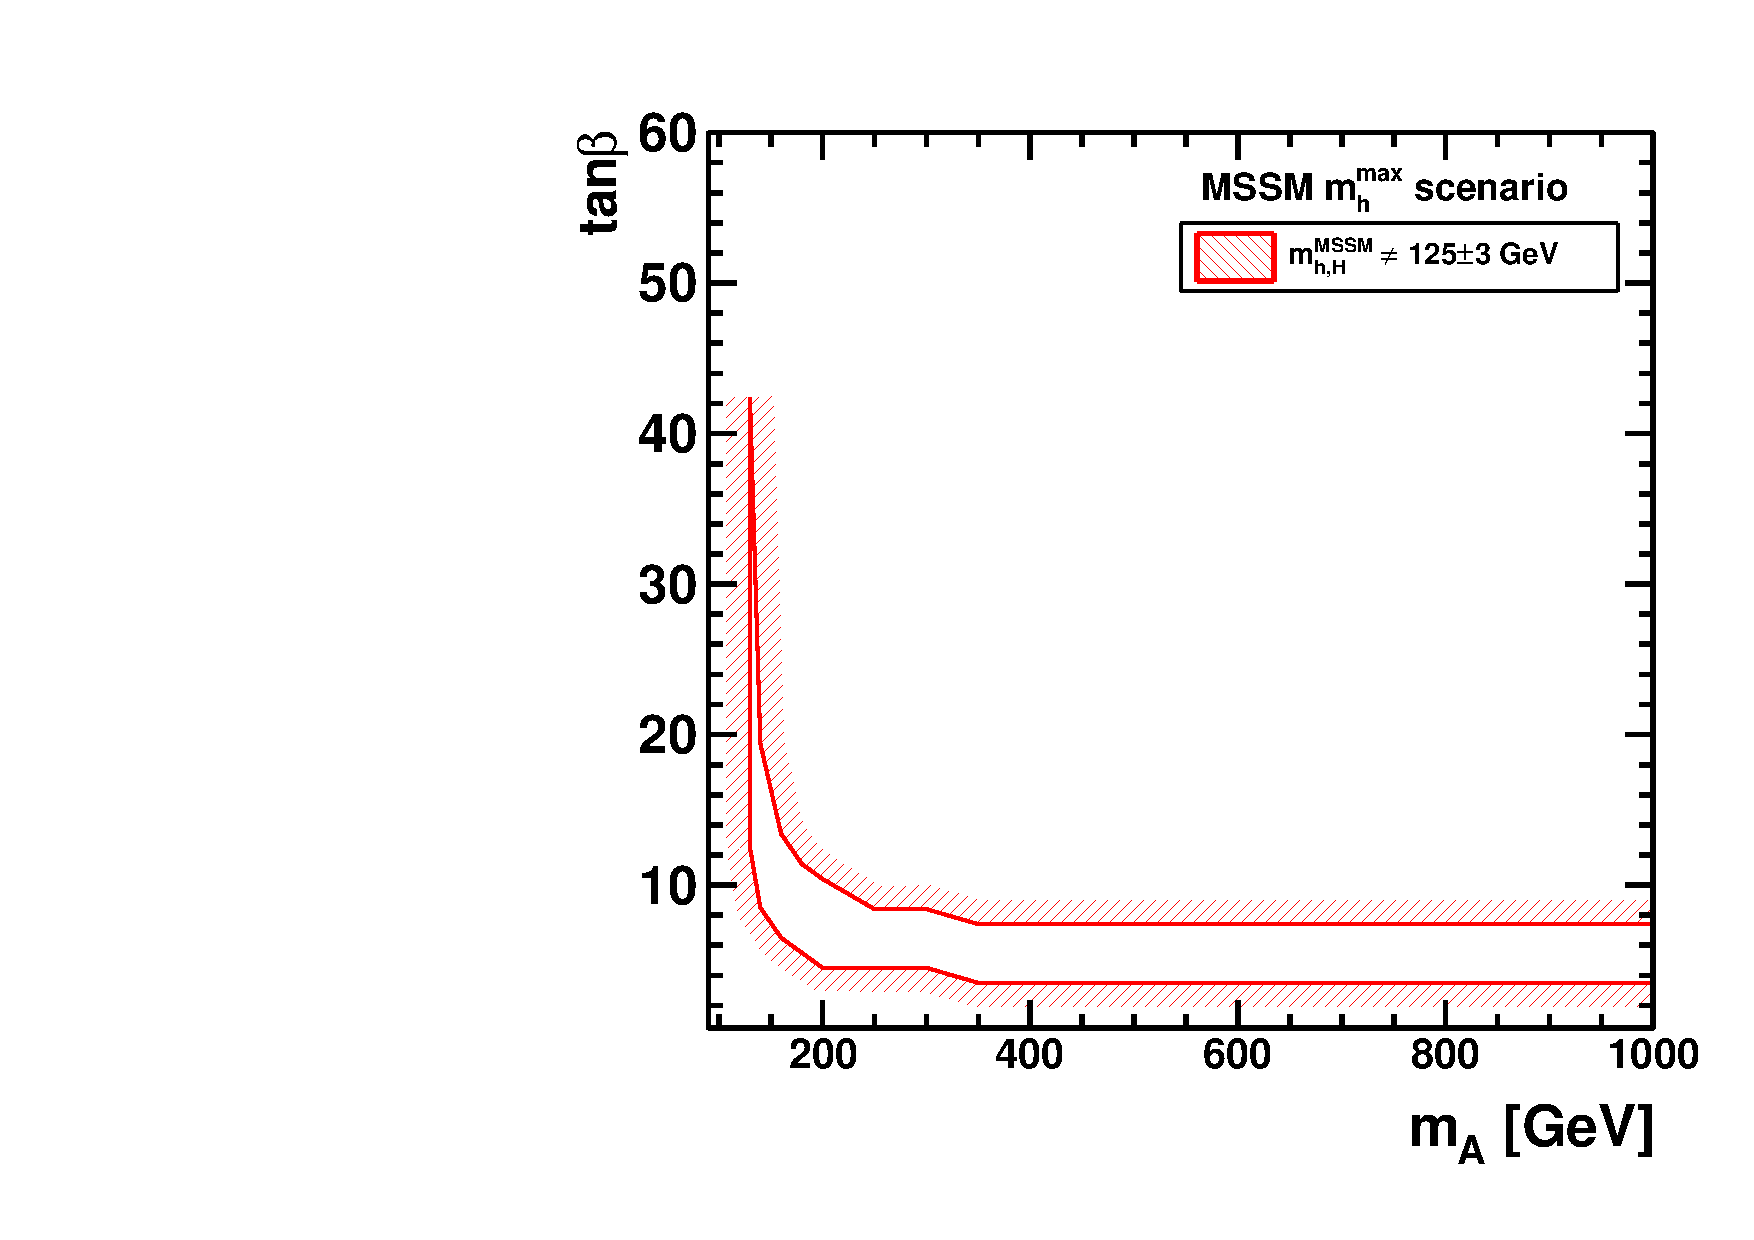
\includegraphics[width=0.5\textwidth]{plots/theory/cmb_mhmax-HypoTest.pdf}
\caption[Region of $m_{\PA}$-$\tan\beta$ space which yields a scalar Higgs mass 
consistent with $125~\GeV$ in the $m_{h}^{\text{max}}$ scenario.]
{Region of $m_{\PA}$-$\tan\beta$ space which yields a scalar Higgs mass 
consistent with $125~\GeV$ in the $m_{h}^{\text{max}}$ scenario. The majority of
this scenario is ruled out by the discovery of a 125$~\GeV$ Higgs boson at the
LHC.}
\label{fig:mhmaxmass}
\end{figure}

\subsubsection{The $m_{h}^{\text{mod}}$ scenario}
\label{sec:mhmodscenario}

As the name suggests, the $m_{h}^{\text{mod}}$ is a slightly modified version of
the $m_{h}^{\text{max}}$, such that the mass of the light Higgs is consistent
with $125~\GeV$ over a much wider range of phase space. This is achieved by
decreasing the ratio of the stop mixing parameter and the masses of the third
generation squarks, $|X_{\Pqt}/M_{\text{SUSY}}|$. In the $m_{h}^{\text{mod+}}$
scenario, the stop mixing is positive, $X_{\Pqt} = 1.5 \cdot M_{\text{SUSY}}$,
which gives better agreement with the experimental measurements of $(g-2)_{\mu}$
\cite{Miller:2007kk}. In the $m_{h}^{\text{mod-}}$ scenario, the stop mixing parameter is
negative, $X_{\Pqt} = -1.9 \cdot M_{\text{SUSY}}$, which results in a
BR($\Pqb\to\Pqs\Pphoton$) with better agreement with measurements
\cite{Lees:2012wg}.

Figure \ref{fig:mhmodmass} indicates the region of parameter space which yields
a Higgs consistent with $125~\GeV$. It can be seen that the area is a lot larger
than in the $m_{h}^{\text{max}}$ case. In all subsequent scenarios, the allowed
region is very similar, excluding only very low $\tan\beta$ values. For the
other scenarios these allowed regions are shown in chapter~\ref{chap:htt-mssm},
in the context of the results of the MSSM $\Pphi \to \Pgt\Pgt$ analysis which
are interpreted in these scenarios.

\begin{figure}[htbp]
\subfloat[]{
   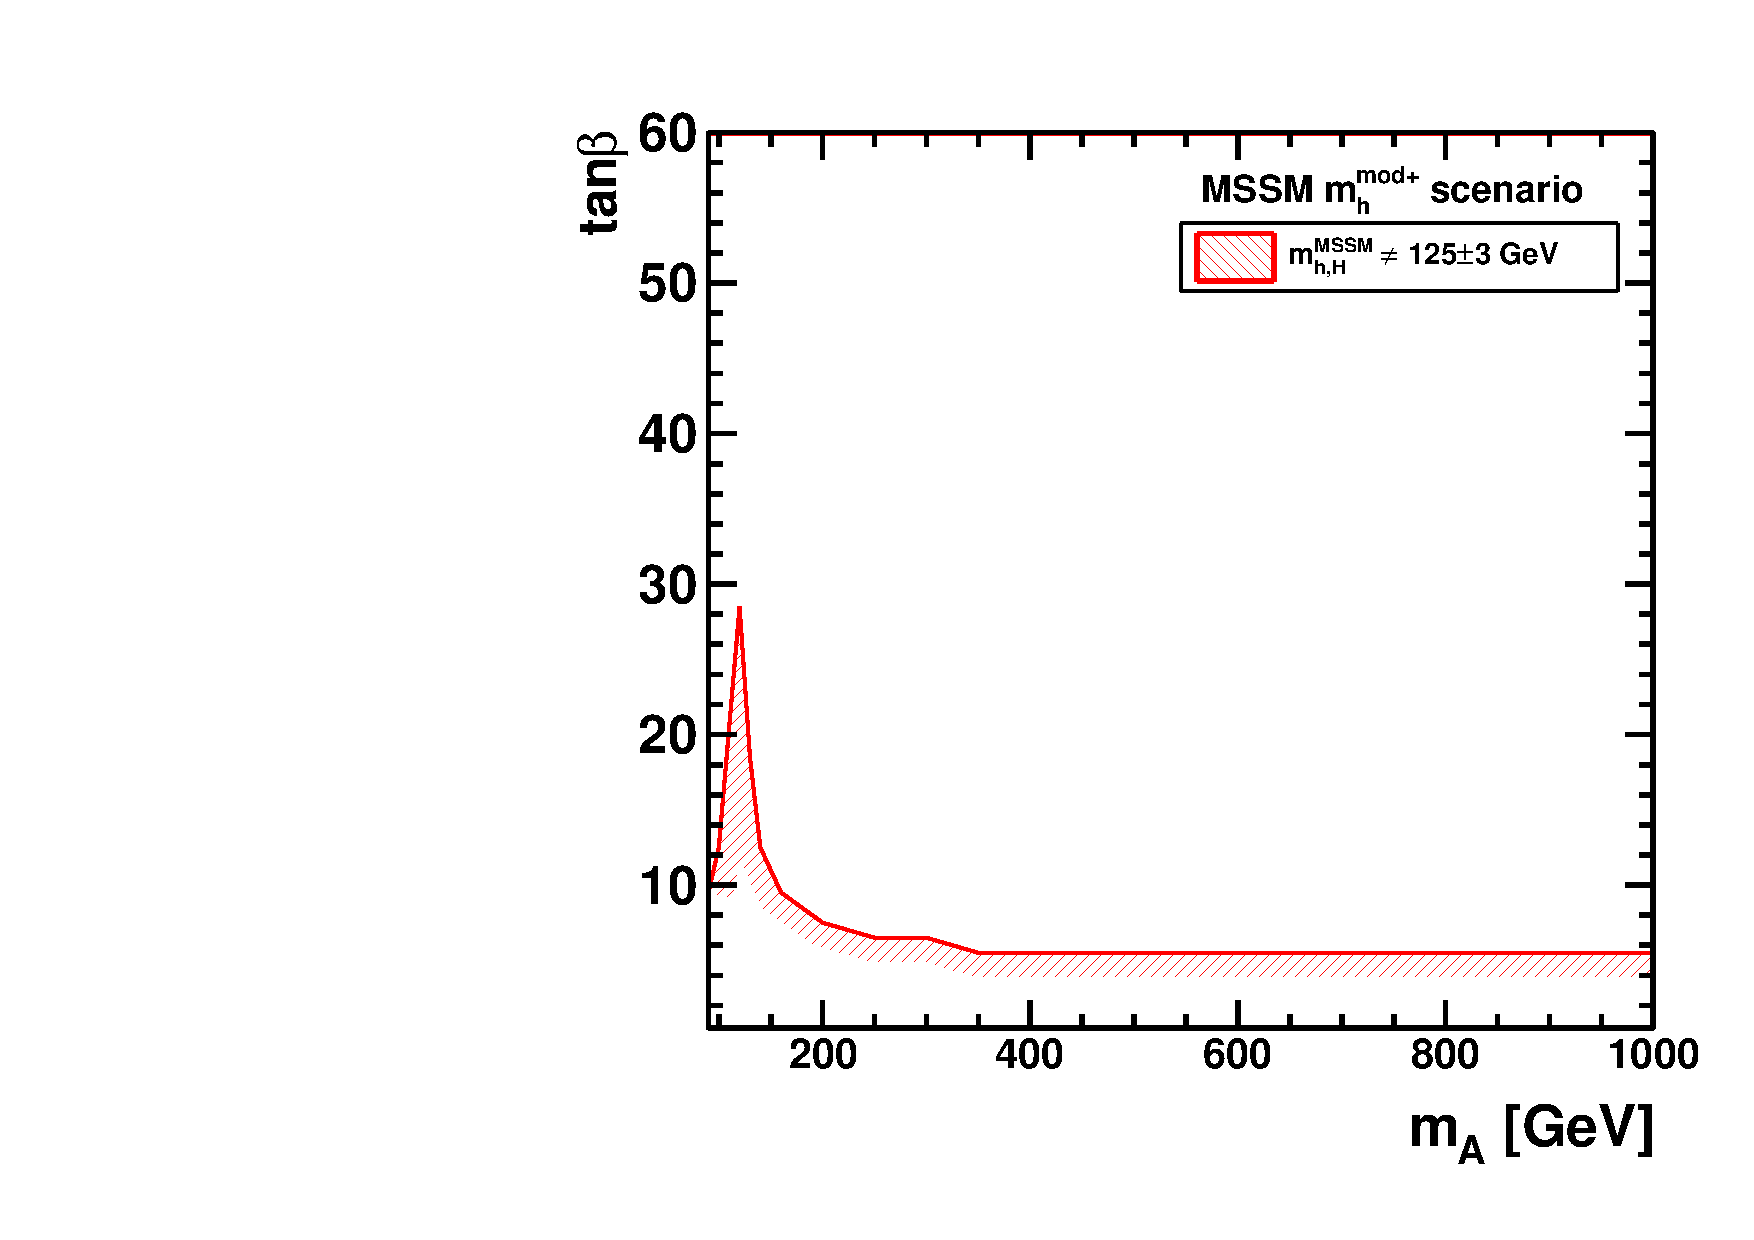
\includegraphics[width=0.5\textwidth]{plots/theory/cmb_mhmodp-HypoTest.pdf}}
\subfloat[]{
   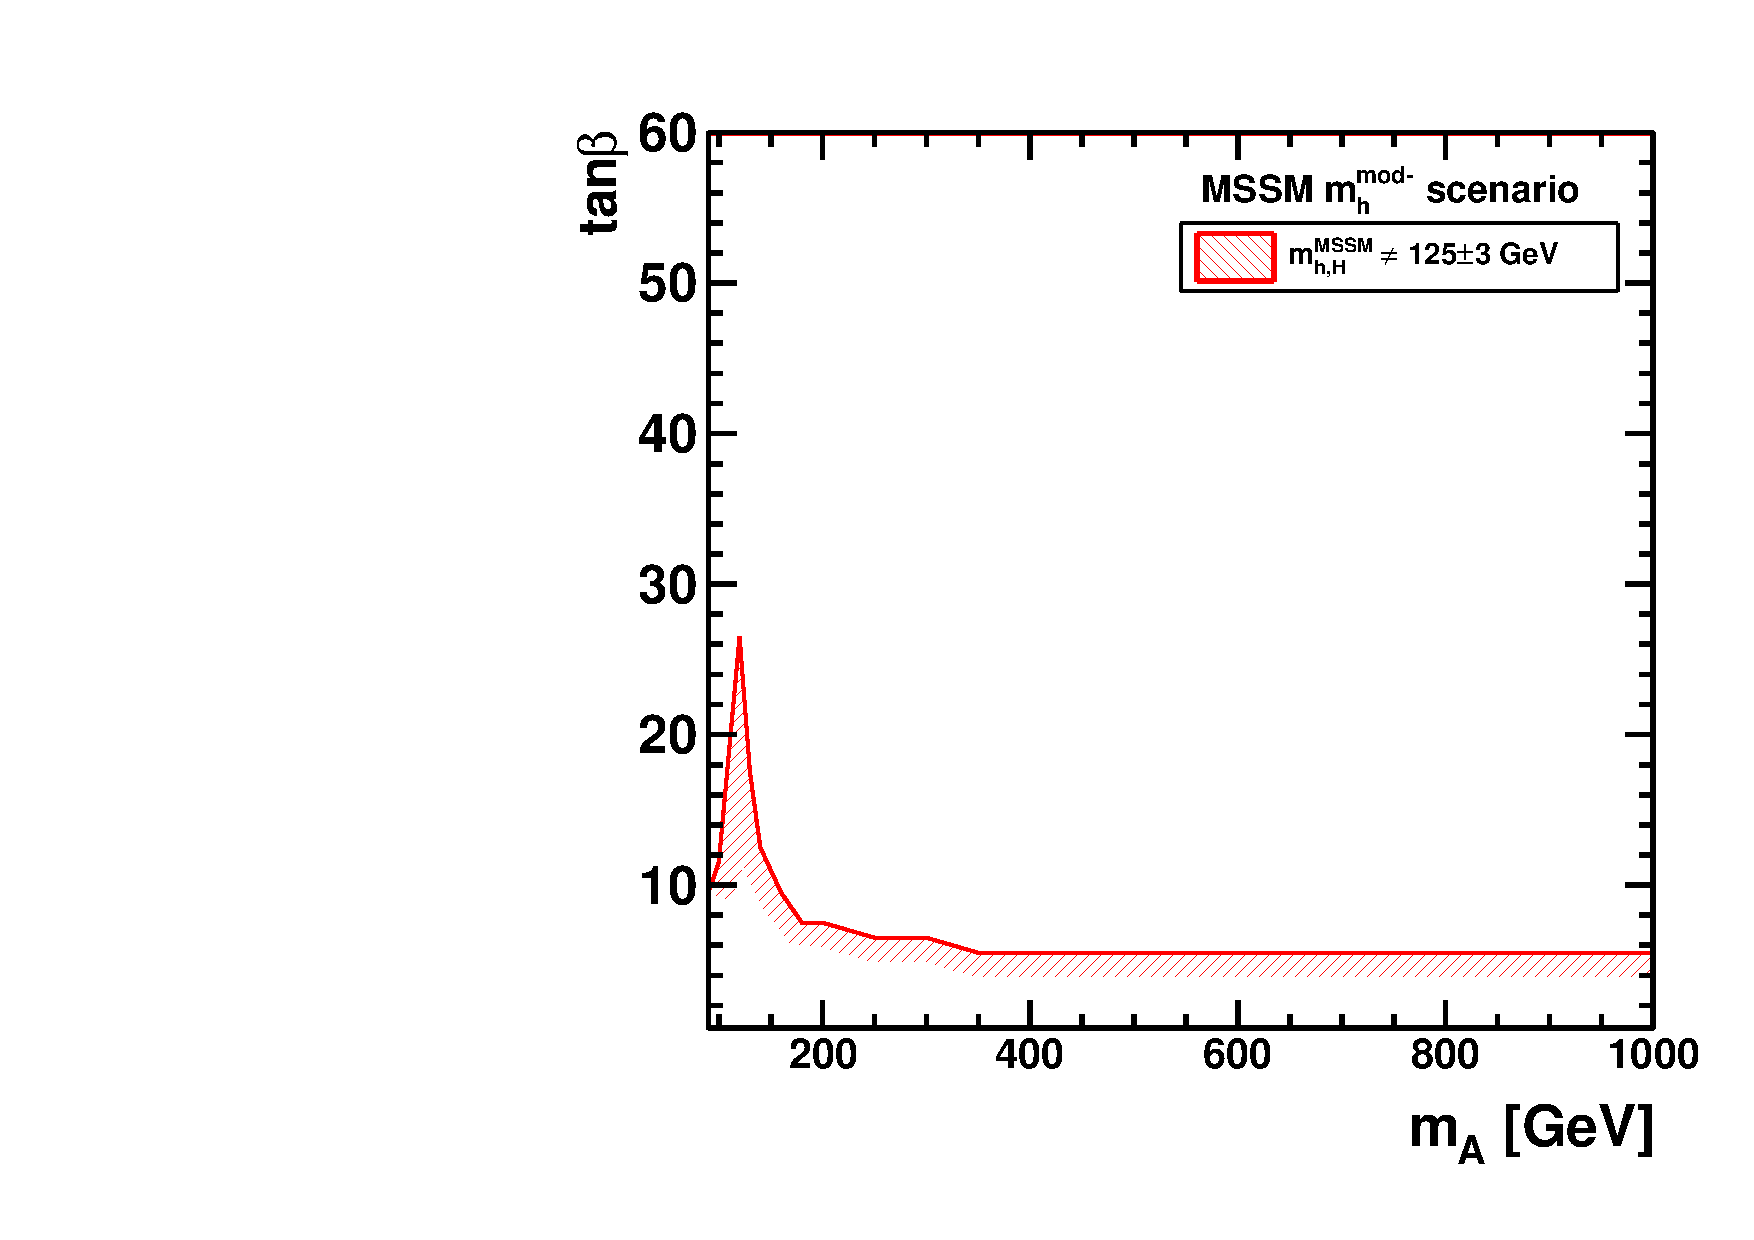
\includegraphics[width=0.5\textwidth]{plots/theory/cmb_mhmodm-HypoTest.pdf}}
\caption[Region of $m_{\PA}$-$\tan\beta$ space which yields a scalar Higgs mass 
consistent with $125~\GeV$ in the $m_{h}^{\text{mod}}$ scenarios.]
{Region of $m_{\PA}$-$\tan\beta$ space which yields a scalar Higgs mass 
consistent with $125~\GeV$ in the $m_{h}^{\text{mod+}}$ (left) and
$m_{h}^{\text{mod-}}$ (right) scenarios. In such modified scenarios, the
majority of phase space is consistent with the discovery of a $125~\GeV$ Higgs.}
\label{fig:mhmodmass}
\end{figure}

\subsubsection{The light stop scenario}
\label{sec:lightstopscenario}

The mass of the lightest CP-even Higgs depends logarithmically on the stop mass,
and therefore a value of $125~\GeV$ can be reached even with values of
$M_{\text{SUSY}} < 1~\TeV$, provided the mixing in the stop sector is large. This
leads to light stops, which could modify the gluon-fusion Higgs production rate.
Such a scenario is referred to as the light-stop scenario. This scenario is
defined to be in agreement with current results of direct searches for stops.
Note that in this scenario $M_{1}$ and $M_{2}$ are not related by the GUT
relation in equation~\ref{eq:GUTrelation}. 
%An assumption used for the calculation of cross-sections in this scenario assumes
%that $m_{\PH} < 2\times $

\subsubsection{The light stau scenario}
\label{sec:lightstauscenario}

The light stau scenario is motivated by the excess of events in the decay
channel of the $\PH\to\Pphoton\Pphoton$ measured by ATLAS
\cite{ATLAS-CONF-2013-012}. Light staus
lead to a modification of the ratio of the lightest Higgs boson decaying into
two photons with respect to the \ac{SM} expectation:
\begin{equation}
r_{\Pphoton\Pphoton} =
\frac{\Gamma(\Ph\to\Pphoton\Pphoton)_{\text{MSSM}}}{\Gamma(\Ph\to\Pphoton\Pphoton)_{\text{SM}}}
.
\end{equation}

For high values of $\tan\beta$ and $m_{\PA}$ this ratio can be as high as 1.3. 

\subsubsection{The $\Pgt$-phobic scenario}
\label{sec:tauphobicscenario}

Similarly to the case of the light stau scenario, the $\Pgt$-phobic scenario is
motivated by the possibility to allow reduced couplings to down-type fermions.
In high $\tan\beta$ and $m_{\PA}$, the ratios:
\begin{equation}
r_{\Pqb\Pqb} =
\frac{\Gamma(\Ph\to\Pqb\Pqb)_{\text{MSSM}}}{\Gamma(\Ph\to\Pqb\Pqb)_{\text{SM}}}
, \quad
r_{\Pgt\Pgt} =
\frac{\Gamma(\Ph\to\Pgt\Pgt)_{\text{MSSM}}}{\Gamma(\Ph\to\Pgt\Pgt)_{\text{SM}}}
\end{equation}

can be significantly lower than 1.

\subsubsection{The low-$m_{\PH}$ scenario}
\label{sec:lowmHscenario}

The low-$m_{\PH}$ scenario is somewhat different from the other scenarios due to
the fact that in this scenario, the Higgs boson with mass of $125~\GeV$ is
assumed to be the heavier scalar Higgs $\PH$. This means that the mass of the
pseudoscalar Higgs must be chosen to be not too high, and is fixed at $m_{\PA} =
110~\GeV$. Since $m_{\PA}$ is fixed in this scenario, the 2-D parameter space
for the scan is chosen as $\mu$-$\tan\beta$, with $\mu$ varied between 300 and
$3100~\GeV$ and $\tan\beta$ between 1.5 and 9.5. All the other parameters are
very similar to those in the $\Pgt$-phobic scenario. In this scenario, the
couplings of the lightest Higgs boson $\Ph$ to gauge bosons is significantly
reduced compared with the \ac{SM} expectations by a factor 2-10, to ensure that
the \Ph is not already excluded by LEP limits. 

\begin{table}[tbh]
\begin{tabular}{|l|c|c|c|}
\hline
Parameter & $m_{h}^{\text{max}}$ & $m_{h}^{\text{mod+}}$ & $m_{h}^{\text{mod-}}$ \\
\hline
$m_{\PA}$ & $90-1000~\GeV$ & $90-1000~\GeV$ & $90-1000~\GeV$\\
$\tan\beta$ & 0.5-60 & 0.5-60 & 0.5-60 \\
$M_{\text{SUSY}}$ & $1000~\GeV$ & $1000~\GeV$ & $1000~\GeV$\\
$\mu$ & $200~\GeV$ & $200~\GeV$ & $200~\GeV$\\
$M_{1}$ & $(5/3)M_{2}\tan{\theta_{W}}^{2}$ & $(5/3)M_{2}\tan{\theta_{W}}^{2}$ & $(5/3)M_{2}\tan{\theta_{W}}^{2}$\\
$M_{2}$ & $200~\GeV$ & $200~\GeV$ & $200~\GeV$ \\
$X_{\Pgt}$ & $2M_{\text{SUSY}}$ & $1.5M_{\text{SUSY}}$ & $-1.9M_{\text{SUSY}}$ \\
$A_{\Pqb},A_{\Pqt},A_{\Pgt}$ & $A_{\Pqb} = A_{\Pqt} = A_{\Pgt}$ & $A_{\Pqb} = A_{\Pqt} = A_{\Pgt}$ & $A_{\Pqb} = A_{\Pqt} = A_{\Pgt}$\\
$m_{\PSgluino}$ & $1500~\GeV$ & $1500~\GeV$ & $1500~\GeV$\\
$m_{\PSlepton_{3}}$ & $1000~\GeV$ & $1000~\GeV$ & $1000~\GeV$\\
\hline
\end{tabular}
\begin{tabular}{|l|c|c|c|c|}
\hline
Parameter & light-stop & light-stau & $\Pgt$-phobic & low-$m_{\PH}$ \\
\hline
$m_{\PA}$ & $90-1000~\GeV$ & $90-1000~\GeV$ & $90-1000~\GeV$ & $110~\GeV$\\
$\tan\beta$ & 0.7-60 & 0.5-60 & 0.9-50 & 1.5-9.5\\
$M_{\text{SUSY}}$ & $500~\GeV$ & $1000~\GeV$ & $1500~\GeV$ & $1500~\GeV$\\
$\mu$ & $400~\GeV$ & $500~\GeV$ & $2000~\GeV$ & $300-3100~\GeV$\\
$M_{1}$ & $340~\GeV$ & $(5/3)M_{2}\tan{\theta_{W}}^{2}$ & $(5/3)M_{2}\tan{\theta_{W}}^{2}$  & $(5/3)M_{2}\tan{\theta_{W}}^{2}$ \\
$M_{2}$ & $400~\GeV$ & $200~\GeV$ & $200~\GeV$ & $200~\GeV$\\
$X_{\Pgt}$ & $2M_{\text{SUSY}}$ & $1.6M_{\text{SUSY}}$ & $2.45M_{\text{SUSY}}$ & $2.45M_{\text{SUSY}}$ \\
$A_{\Pqb},A_{\Pqt},A_{\Pgt}$ & $A_{\Pqb} = A_{\Pqt} = A_{\Pgt}$ & $A_{\Pqb} = A_{\Pqt}, A_{\Pgt} = 0$ & $A_{\Pqb} = A_{\Pqt} = A_{\Pgt}$ & $A_{\Pqb} = A_{\Pqt} = A_{\Pgt}$ \\
$m_{\PSgluino}$ & $1500~\GeV$ & $1500~\GeV$  & $1500~\GeV$ & $1500~\GeV$ \\
$m_{\PSlepton_{3}}$ & $1000~\GeV$ & $245~\GeV$ & $500~\GeV$ &  $1000~\GeV$ \\
\hline
\end{tabular}
\caption[Parameters defining the $m_{h}^{\text{max}}$, $m_{h}^{\text{mod+}}$,
$m_{h}^{\text{mod-}}$, light-stop, light-stau, $\Pgt$-phobic and
low-$m_{\PH}$ MSSM benchmark scenarios.]{Parameters defining the $m_{h}^{\text{max}}$, $m_{h}^{\text{mod+}}$,
$m_{h}^{\text{mod-}}$, light-stop, light-stau, $\Pgt$-phobic and
low-$m_{\PH}$ MSSM benchmark scenarios \cite{HIG-13-021}.}
\label{tab:mssmbenchmarks}
\end{table}

\subsection{Modification of MSSM models at low $\tan\beta$}
\label{sec:lowtanbscenario}

In all of the scenarios discussed in the previous sections, the mass of either
the lighter or heavier scalar Higgs boson is consistent with $125~\GeV$ over a
wide range of phase space. However, one thing common to all of these scenarios
is the fact that in general the mass is not consistent at very low $\tan\beta$
values, where the mass of the lightest Higgs becomes too light to be consistent
with $125~\GeV$. As results such as those discussed in chapter~\ref{chap:htt-mssm} 
rule out larger regions of phase space at high $\tan\beta$, attention turns to this low
$\tan\beta$ region and analyses which could access it.

The low $\tan\beta$ region can be re-opened if the value of $M_{\text{SUSY}}$ is
allowed to be higher than $1~\TeV$ \cite{Djouadi:2013vqa}. In the \ac{MSSM}, values of
$M_{\text{SUSY}}$ must be lower than $3~\TeV$ to avoid too much fine tuning in
the model. However, as searches at the LHC have yet to discover supersymmetric
particles, it is natural that models with higher SUSY scales are being
considered, and as the allowed amount of fine-tuning in a model is somewhat
subjective, attention is turning more to these types of scenarios. Figure
\ref{fig:MSUSYcontours} illustrates the mass of the $\Ph$ boson at different
choices of $M_{\text{SUSY}}$ for a range of $\tan\beta$ values. It can be seen
that $m_{\Ph} = 125\pm 3~\GeV$ can be achieved for values of $\tan\beta$ as low
as $1~\GeV$ if $M_{\text{SUSY}}$ is allowed to be in the range $100-1000~\TeV$.
Slightly higher $\tan\beta$ values in the range 2--5 can be achieved with
$M_{\text{SUSY}}$ values only as high as a few $\TeV$. 

\begin{figure}[htbp]
   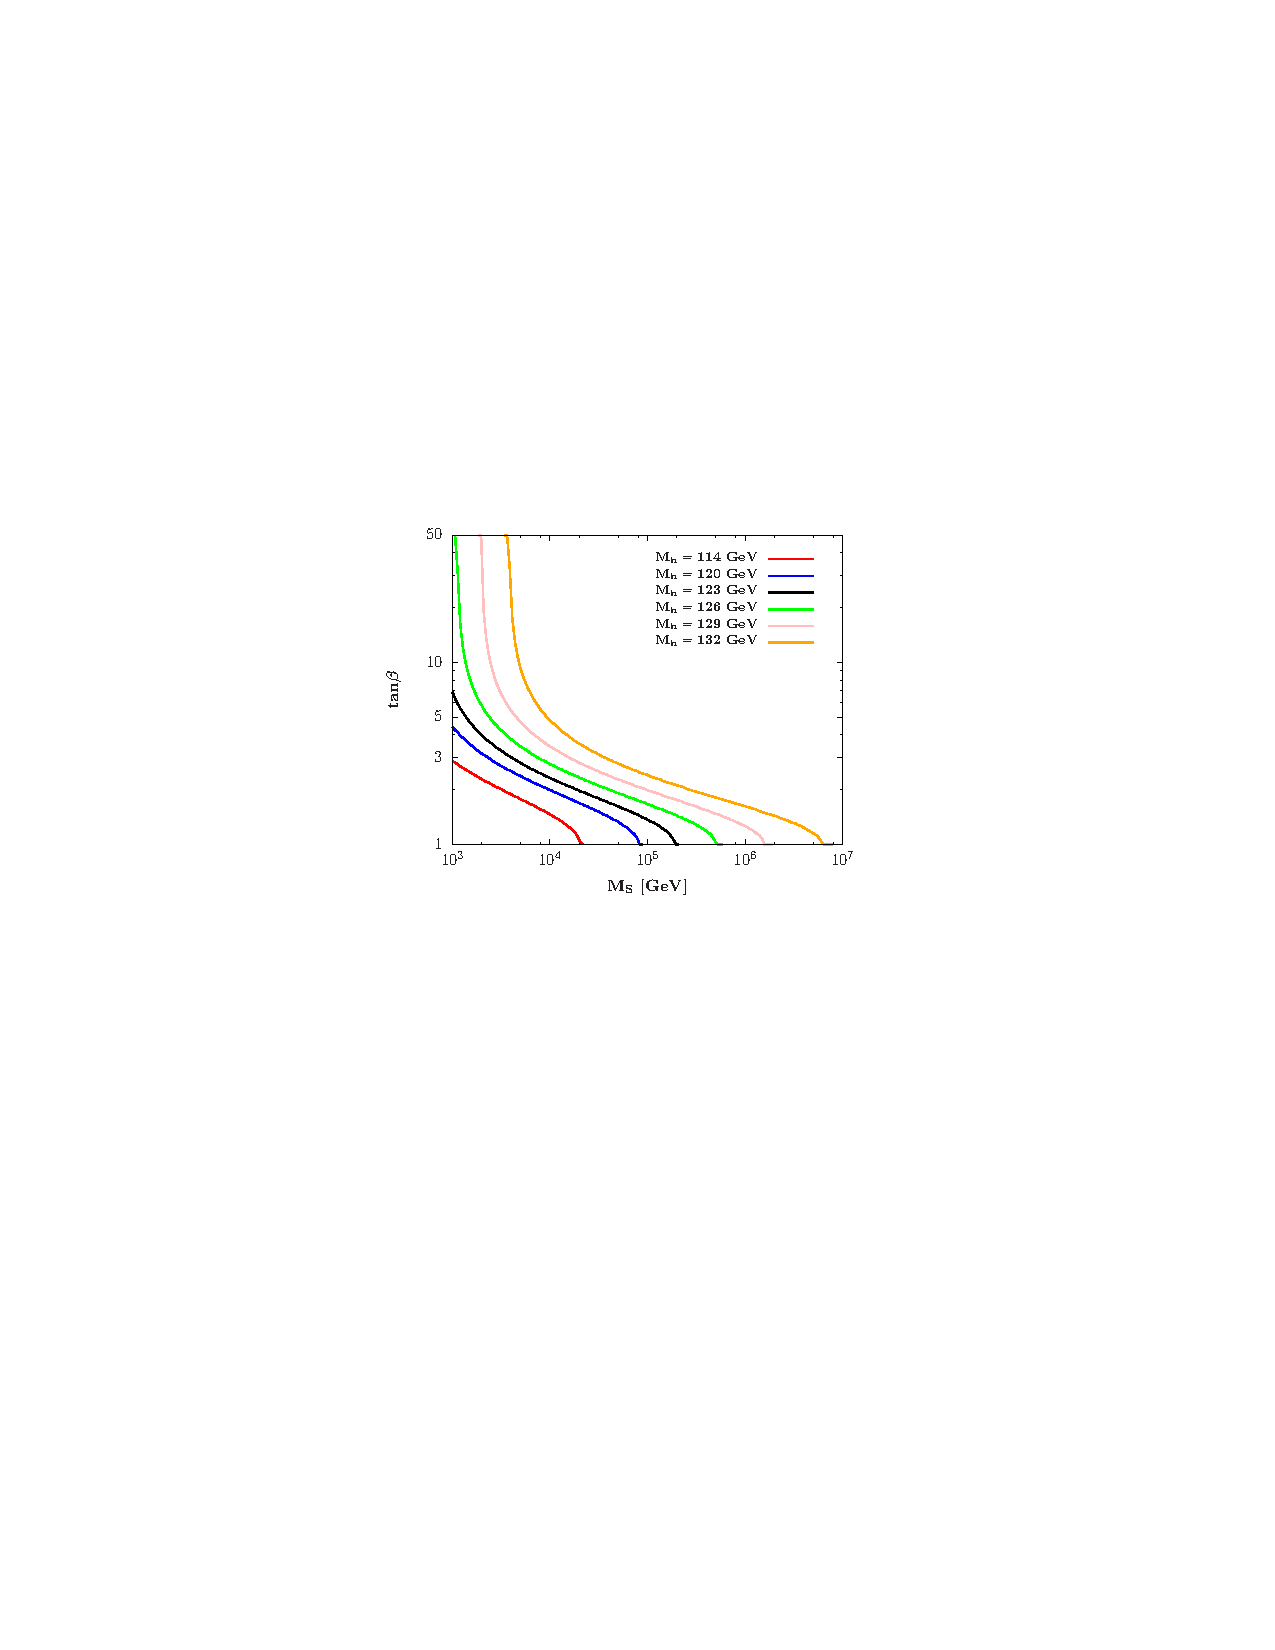
\includegraphics[width=0.7\textwidth]{plots/theory/MSUSY_tanb.pdf}
\caption[Contours in the $M_{\text{SUSY}}$-$\tan\beta$ plane for
constant $m_{\Ph}$ values around $125~\GeV$.]{Contours in the $M_{\text{SUSY}}$($M_{S}$)-$\tan\beta$ plane for
constant $m_{\Ph}$ values around $125~\GeV$, illustrating that higher
$M_{\text{SUSY}}$ values can allow a light Higgs consistent with $125~\GeV$ for
even very low $\tan\beta$ values \cite{Djouadi:2013vqa}.}
\label{fig:MSUSYcontours}
\end{figure}

In such a low $\tan\beta$ region, the gluon fusion production process dominates
over any b-associated production. Figure~\ref{fig:XSlowtanb} indicates the
production cross-sections for each of the neutral Higgs bosons in such a low
$\tan\beta$ regime for $\sqrt{s}=8~\TeV$. It can be seen that the production of
the heavier $\PA$ and $\PH$ bosons via gluon fusion dominates over any of the
other production mechanisms. Thus to access information about such a scenario,
the heavier Higgs bosons with masses up to $1~\TeV$ must be searched for.
Figure~\ref{fig:BRlowtanb} illustrates the branching ratios of the $\PA$ and
$\PH$ bosons in such a mass range. 

\begin{figure}[htbp]
   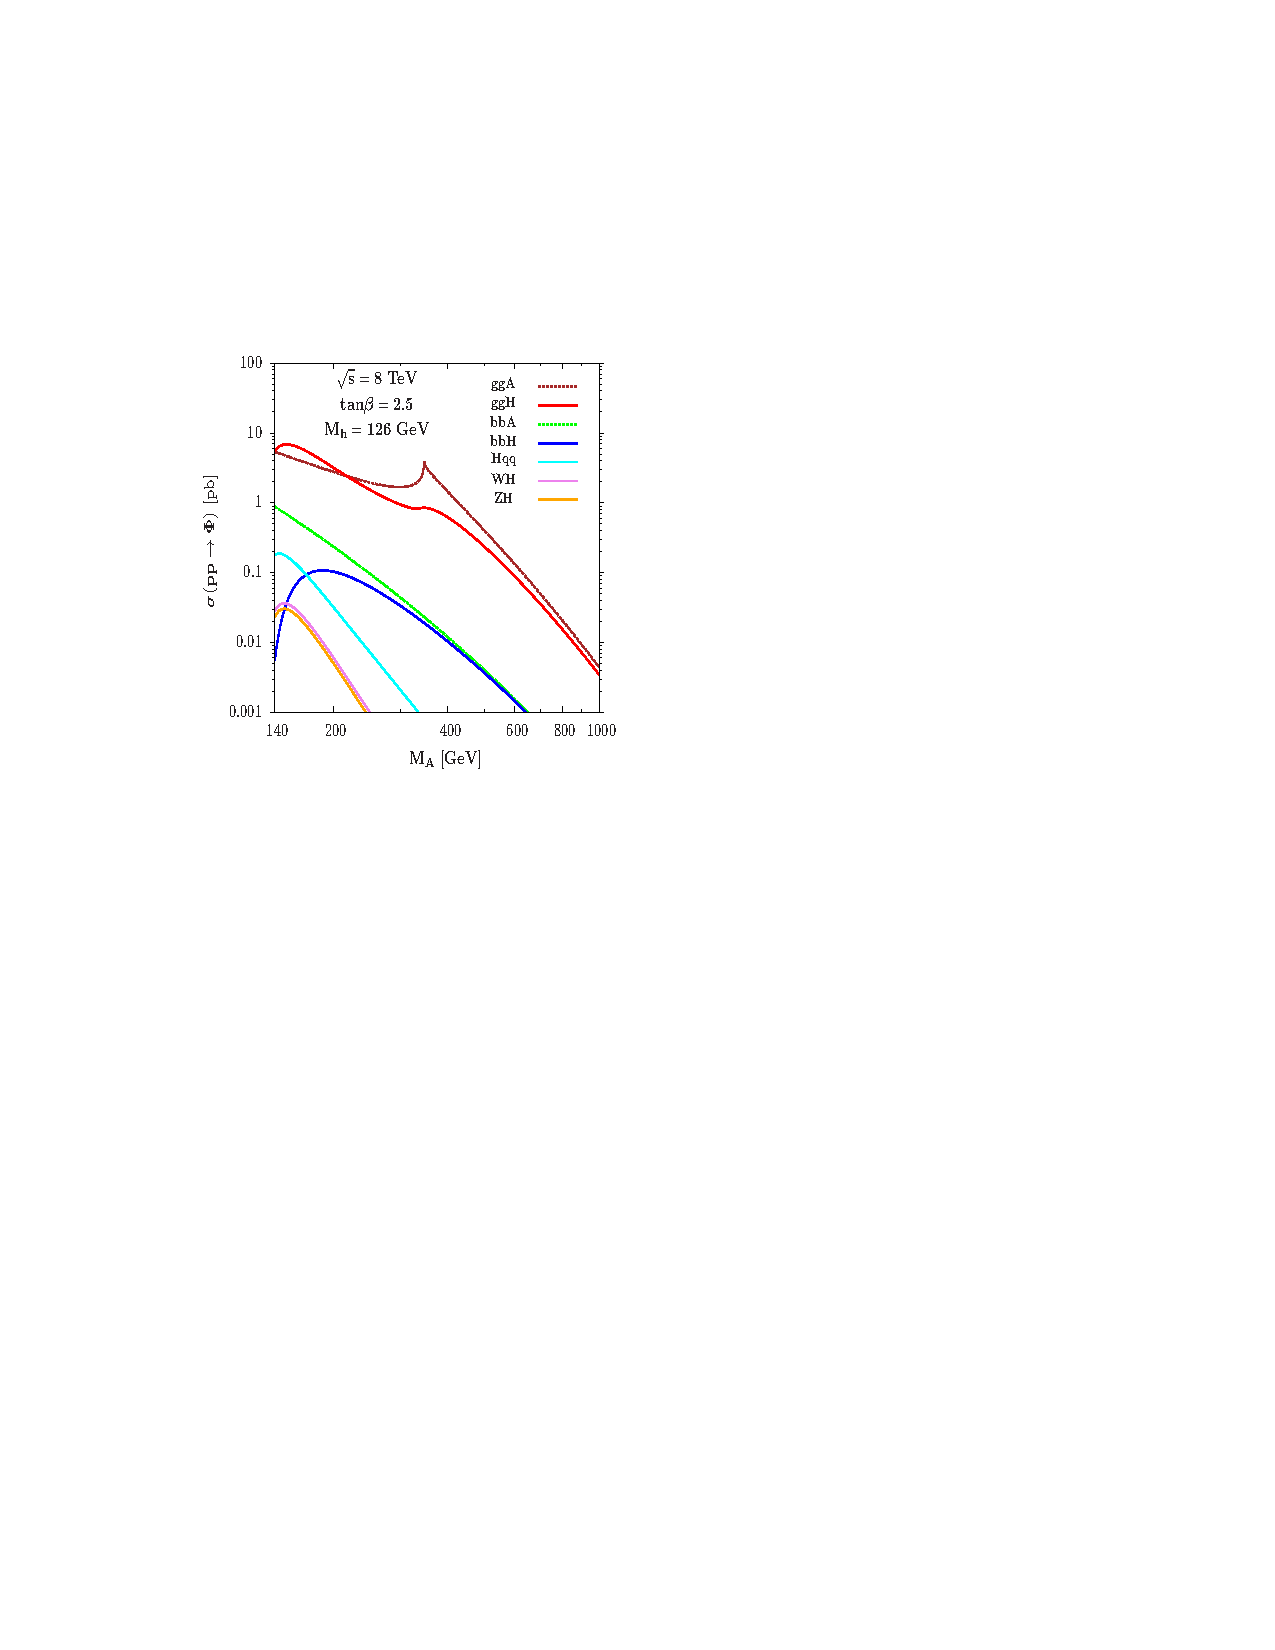
\includegraphics[width=0.5\textwidth]{plots/theory/XS_lowtanb.pdf}
\caption[Cross-sections for the production of the three neutral Higgs bosons in
the low $\tan\beta$ regime.]{Cross-sections for the production of the three neutral Higgs bosons in
the low $\tan\beta$ regime. The production of the $\PH$ and $\PA$ bosons
via gluon fusion dominates over any of the other production processes \cite{Djouadi:2013vqa}.}
\label{fig:XSlowtanb}
\end{figure}

\begin{figure}[htbp]
   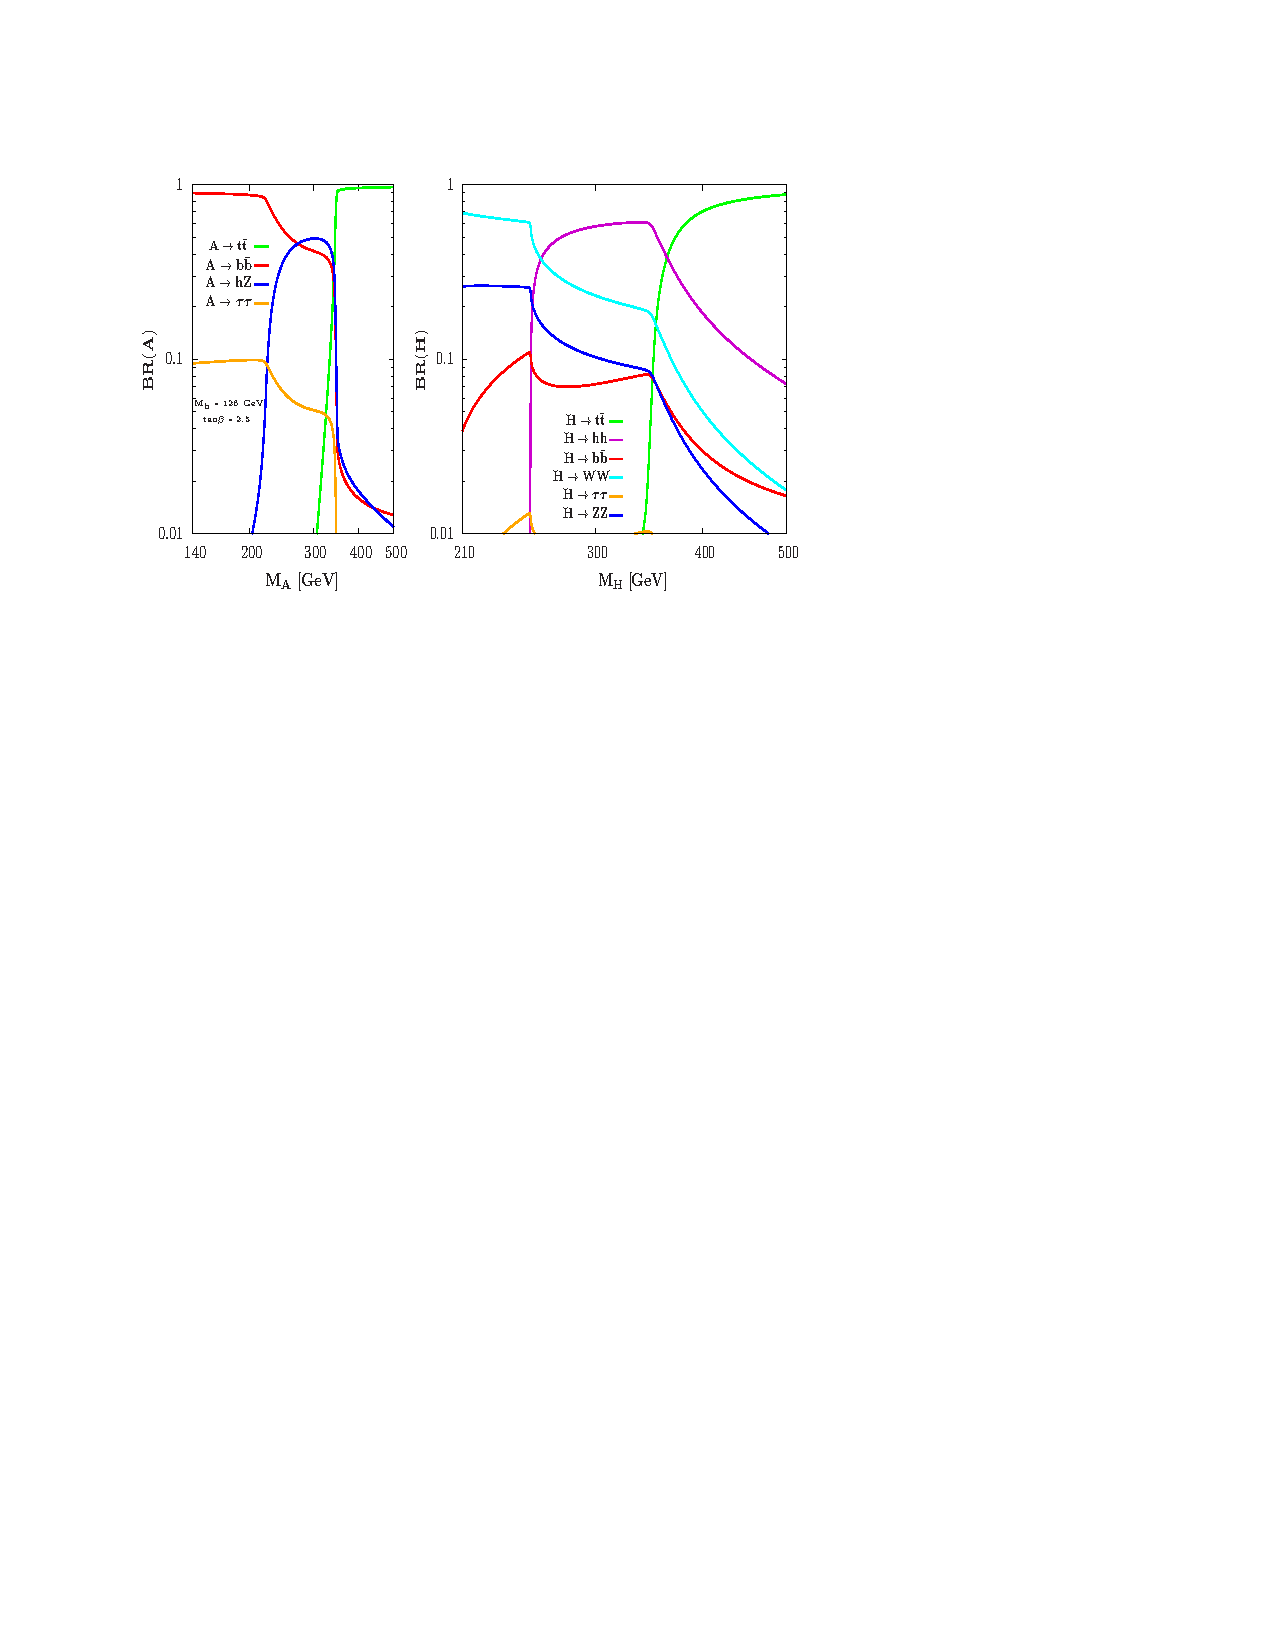
\includegraphics[width=0.7\textwidth]{plots/theory/BR_lowtanb.pdf}
\caption[Branching ratios for the $\PH$ and $\PA$ bosons in the low $\tan\beta$
regime.]{Branching ratios for the $\PH$ and $\PA$ bosons in the low $\tan\beta$
regime \cite{Djouadi:2013vqa}.}
\label{fig:BRlowtanb}
\end{figure}

From figure \ref{fig:BRlowtanb}, it can be seen that in the central region of 
$m_{\PA}-\tan\beta$ space, branching ratios for the decays of
$\PH\to\Ph\Ph$ and $\PA\to\PZ\Ph$ are enhanced. Several recent LHC analyses have
made searches for these decays in the scenario where the $\Ph$ is the $125~\GeV$
Higgs discovered at the LHC. Various final states have been studied including
for the $\PH\to\Ph\Ph$ analysis $\Pphoton\Pphoton\Pqb\Pqb$ \cite{Aad:2014yja,CMS-PAS-HIG-13-032} and 
$\Pqb\Pqb\Pqb\Pqb$ \cite{CMS-PAS-HIG-14-013} and for the $\PA\to\PZ\Ph$ analysis $\ell\ell\Pqb\Pqb$
and $\ell\ell\Pgt\Pgt$ \cite{Aad:2015wra,CMS-PAS-HIG-14-011}. 
Chapter~\ref{chap:Hhh} documents a $\PH\to\Ph\Ph$ analysis in the
final state of $\Pgt\Pgt\Pqb\Pqb$. Such results can be interpreted in an
appropriate low $\tan\beta$ scenario or in a more general Two Higgs Doublet
Model (2HDM).
 



